
%\begin{frame}{Edit Distance}
%
%  \begin{block}{Edit distance $\ed(X,Y)$ \hfill Levenshtein distance [Lev65]}
%      Minimum number of character insertions, deletions, and substitutions that transform $X$ to $Y$.
%  \end{block}
%  
%  \begin{center}
%  \begin{tikzpicture}
%    
%    \begin{scope}[xscale=0.3,yscale=-1]
%    \draw (-1,0) node{$X:$};
%    \draw (-1,1) node{$Y:$};
%    \foreach \x [count=\i] in {b,\textcolor{red}{b},a,b,a,b,\textcolor{red}{b},a,a,b}{
%      \draw (\i,0) node {$\mathtt{\vphantom{ab}\x}$};
%    }
%    \foreach \x [count=\i] in {b,a,b,a,b,\textcolor{red}{a},a,a,b,\textcolor{red}{b}}{
%        \draw (\i,1) node {$\mathtt{\vphantom{ab}\x}$};
%    }
%    \foreach \x/\y in {1/1,3/2,4/3,5/4,6/5,8/7,9/8,10/9}{
%      \draw[thick] (\x,0.2) -- (\y,0.9);
%    }
%    \foreach \x/\y in {7/6}{
%      \draw[thick,red,densely dashed] (\x,0.2) -- (\y,0.9);
%    }
%  
%  
%    \draw (20,0.5) node {$\ed(X,Y)=3$};
%    \end{scope}
%  \end{tikzpicture}
%  \end{center}
%  
%  \end{frame}


\begin{frame}{Weighted Edit Distance}
    \vfill
    \begin{block}{Weighted Edit Distance $\wed(X,Y)$ \hfill $w \colon (\Sigma \cup \{\varepsilon\}) \times (\Sigma \cup \{\varepsilon\}) \to \RR_{\ge 0}$}
        The minimum cost of transforming $X$ into $Y$ by editing individual characters, where:
        \begin{itemize}
            \item inserting $b$ costs $w(\varepsilon, b)$;
            \item deleting $a$ costs $w(a, \varepsilon)$;
            \item substituting $a$ for $b$ costs $w(a, b)$.
        \end{itemize}
    \end{block}
  
  %\begin{center}
%\begin{tikzpicture}
%    \matrix[matrix of nodes,
%    nodes={minimum size=6mm, text centered, draw, font=\bfseries},
%    column sep=-\pgflinewidth, row sep=-\pgflinewidth,
%    nodes in empty cells,
%    anchor=north west
%  ] (m) at (0,0) {
%    w & $\varepsilon$ & $a$ & $b$ \\
%    $\varepsilon$ & 0 & 1 & 3 \\
%    $a$ & 1 & 0 & 2 \\
%    $b$ & 3 & 2 & 0 \\
%  };
%\end{tikzpicture}
    \vspace*{0.5cm}
  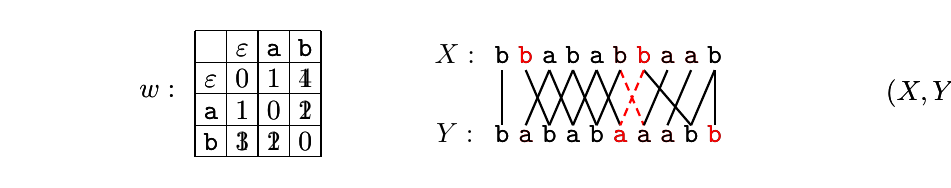
\begin{tikzpicture}
      \hspace*{1.3cm}
    \begin{scope}[xscale=0.3,yscale=-1]
    %\matrix (first) [table,text width=6em]
    %\matrix[matrix of nodes,
    %      nodes={draw, minimum size=10mm, anchor=center},
    %      column sep=-\pgflinewidth, row sep=-\pgflinewidth] (m) {
    
    %    1 & 2 & 3 \\
    %    4 & 5 & 6 \\
    %    7 & 8 & 9 \\
    %};
    
    %\matrix (m) at (-10, 0) {
    %\node{3} & \node{2} \\
    %\node{4} & \node{5} \\
    %};
    \def\st{10}
    \def\sx{\st-12}
    \def\sy{-0.3}
    \def\sizx{1.3333333}
    \def\sizy{0.4}
    \foreach \x in {0,1,2,3,4}{
        \draw (\sx + \sizx * \x, \sy) -- (\sx + \sizx * \x, \sy + \sizy * 4);
    }
    \foreach \y in {0,1,2,3,4}{
        \draw (\sx, \sy + \sizy * \y) -- (\sx + \sizx * 4, \sy + \sizy * \y);
    }
    \foreach \ch/\r/\c in {w:/1.3/-1.7,\varepsilon/0/1,\mathtt{a}/0/2,\mathtt{b}/0/3,\varepsilon/1/0,0/1/1,1/1/2,4/1/3,\mathtt{a}/2/0,1/2/1,0/2/2,2/2/3,\mathtt{b}/3/0,3/3/1,2/3/2,0/3/3}{
        \draw<1> (\sx + \sizx * \c + \sizx * 0.5, \sy + \sizy * \r + \sizy * 0.5) node {$\mathtt{\vphantom{ab}}\ch$};
    }
    \foreach \ch/\r/\c in {w:/1.3/-1.7,\varepsilon/0/1,\mathtt{a}/0/2,\mathtt{b}/0/3,\varepsilon/1/0,0/1/1,1/1/2,1/1/3,\mathtt{a}/2/0,1/2/1,0/2/2,1/2/3,\mathtt{b}/3/0,1/3/1,1/3/2,0/3/3}{
        \draw<2-> (\sx + \sizx * \c + \sizx * 0.5, \sy + \sizy * \r + \sizy * 0.5) node {$\mathtt{\vphantom{ab}}\ch$};
    }
    

    \draw (\st-1,0) node{$X:$};
    \draw (\st-1,1) node{$Y:$};

    \foreach \x [count=\i] in {b,b,a,b,a,\textcolor{red}{b},b,\textcolor{red}{a},\textcolor{red}{a},b}{
      \draw<1> (\st+\i,0) node {$\mathtt{\vphantom{ab}\x}$};
    }
    \foreach \x [count=\i] in {b,\textcolor{red}{a},b,a,b,a,\textcolor{red}{a},\textcolor{red}{a},b,b}{
        \draw<1> (\st+\i,1) node {$\mathtt{\vphantom{ab}\x}$};
    }
    \foreach \x/\y in {1/1,2/3,3/4,4/5,5/6,7/9,10/10}{
      \draw<1>[thick] (\st+\x,0.2) -- (\st+\y,0.9);
    }
    \foreach \x/\y in {6/7}{
      \draw<1>[thick,red,densely dashed] (\st+\x,0.2) -- (\st+\y,0.9);
    }
    

    \foreach \x [count=\i] in {b,\textcolor{red}{b},a,b,a,b,\textcolor{red}{b},a,a,b}{
      \draw<2-> (\st+\i,0) node {$\mathtt{\vphantom{ab}\x}$};
    }
    \foreach \x [count=\i] in {b,a,b,a,b,\textcolor{red}{a},a,a,b,\textcolor{red}{b}}{
        \draw<2-> (\st+\i,1) node {$\mathtt{\vphantom{ab}\x}$};
    }
    \foreach \x/\y in {1/1,3/2,4/3,5/4,6/5,8/7,9/8,10/9}{
      \draw<2->[thick] (\st+\x,0.2) -- (\st+\y,0.9);
    }
    \foreach \x/\y in {7/6}{
      \draw<2->[thick,red,densely dashed] (\st+\x,0.2) -- (\st+\y,0.9);
    }
    
  
  
    \draw<1> (\st+20,0.5) node {$\wed(X,Y)=6$};
    \draw<2-> (\st+20,0.5) node {$\ed(X,Y)=3$};
    \end{scope}
  \end{tikzpicture}
  \vfill
\end{frame}

\begin{frame}<1>{State of the Art}
    \vspace{-1cm}

\hfill \textbf{\small \boldmath Notation: $n = |X| + |Y|$\onslide<2->{, $k = \wed(X, Y)$}}

\vspace{0.3cm}

\small
\begin{tabular}{rccr}
    \emph{Reference} & \emph{Time} & \emph{Weights} & \onslide<5->{\emph{Matching Lower Bound}}\\[1ex]
    \hline\\[-1.3ex]
    \where{Vin68,NW70,Sel74,WF74} & $\Oh(n^2)$ & any & \onslide<5->{under OVH (or SETH)}\\[1ex]
    \onslide<3->{\where{Ukk85,Mye86} & $\Oh(nk)$ & $\mathbb{R}_{\ge 1}$ & \\[1ex]}
    \onslide<4->{\where{LV88} & $\Oh(n + k^2)$ & $\{1\}$ & \onslide<5->{under OVH, $1 \le k \le n$}\\[1ex]}
    \onslide<6->{\where{DGHKS23} & $\Oh(n + k^5)$ & $\mathbb{R}_{\ge 1}$ & \\[1ex]}
    \onslide<7->{\where{CKW23} & $\tOh(n + \sqrt{nk^3})$ & $\mathbb{R}_{\ge 1}$ & under APSP, $\sqrt{n} \le k \le n$ \\[1ex]}
    \onslide<8->{\thiswork & $\tOh(n + Wk^2)$ & $\{1, 2, \ldots, W\}$ & \hspace{0.3cm}under OVH, $1 \le k \le n$ and $W = n^{o(1)}$}
\end{tabular}

\vfill

\end{frame}


\begin{frame}<1,2,5>{Alignment Graph and the $\Oh(n^2)$-Time Algorithm}

  \begin{center}
    \begin{tikzpicture}[x=0.625cm, y=-0.625cm]
      \draw[white] (-1,-1) -- (11,11);
      \filldraw<6->[line width=7pt,black!20] (0,0)--(3,0) -- (10,7) -- (10,10)-- (7,10) -- (0,3) -- cycle;
      \onslide<2,5->{
      \draw[line width=7pt, blue!30,line cap=round](0,0) -- (1,1) -- (2,1) -- (10,9) -- (10,10);
      \begin{scope}[x=0.3cm,y=-1cm,xshift=7.2cm,yshift=-2.75cm]
        \foreach \x [count=\i] in {b,\textcolor{darkred}{b},a,b,a,b,\textcolor{darkred}{b},a,a,b}{
          \draw (\i,0) node {$\mathtt{\vphantom{ab}\x}$};
        }
        \foreach \x [count=\i] in {b,a,b,a,b,\textcolor{darkred}{a},a,a,b,\textcolor{darkred}{b}}{
            \draw (\i,1) node {$\mathtt{\vphantom{ab}\x}$};
        }
        \foreach \x/\y in {1/1,3/2,4/3,5/4,6/5,8/7,9/8,10/9}{
          \draw[thick,darkgreen] (\x,0.2) -- (\y,0.9);
        }
        \foreach \x/\y in {7/6}{
          \draw[thick,darkred,densely dashed] (\x,0.2) -- (\y,0.9);
        }
      \end{scope}
      }
      \onslide<3>{
        \draw[line width=7pt, blue!30,line cap=round](0,0) -- (1,0) -- (9,8) -- (9,9) -- (10,10);
        \begin{scope}[x=0.3cm,y=-1cm,xshift=7.2cm,yshift=-2.75cm]
          \foreach \x [count=\i] in {\textcolor{darkred}{b},b,a,b,a,b,\textcolor{darkred}{b},a,a,b}{
            \draw (\i,0) node {$\mathtt{\vphantom{ab}\x}$};
          }
          \foreach \x [count=\i] in {b,a,b,a,b,\textcolor{darkred}{a},a,a,\textcolor{darkred}{b},b}{
              \draw (\i,1) node {$\mathtt{\vphantom{ab}\x}$};
          }
          \foreach \x/\y in {2/1,3/2,4/3,5/4,6/5,8/7,9/8,10/10}{
            \draw[thick,darkgreen] (\x,0.2) -- (\y,0.9);
          }
          \foreach \x/\y in {7/6}{
            \draw[thick,darkred,densely dashed] (\x,0.2) -- (\y,0.9);
          }
        \end{scope}
        }
      \onslide<1-3>{
      \bigpicture{\input{graph.tex}}
      }
      \onslide<4->{
        \bigpicture{\input{graphdp.tex}}
        }

    \end{tikzpicture}
  \end{center}
  
\end{frame}

\begin{frame}<1-2>{State of the Art}
    \vspace{-1cm}

\hfill \textbf{\small \boldmath Notation: $n = |X| + |Y|$\onslide<2->{, $k = \wed(X, Y)$}}

\vspace{0.3cm}

\small
\begin{tabular}{rccr}
    \emph{Reference} & \emph{Time} & \emph{Weights} & \onslide<5->{\emph{Matching Lower Bound}}\\[1ex]
    \hline\\[-1.3ex]
    \where{Vin68,NW70,Sel74,WF74} & $\Oh(n^2)$ & any & \onslide<5->{under OVH (or SETH)}\\[1ex]
    \onslide<3->{\where{Ukk85,Mye86} & $\Oh(nk)$ & $\mathbb{R}_{\ge 1}$ & \\[1ex]}
    \onslide<4->{\where{LV88} & $\Oh(n + k^2)$ & $\{1\}$ & \onslide<5->{under OVH, $1 \le k \le n$}\\[1ex]}
    \onslide<6->{\where{DGHKS23} & $\Oh(n + k^5)$ & $\mathbb{R}_{\ge 1}$ & \\[1ex]}
    \onslide<7->{\where{CKW23} & $\tOh(n + \sqrt{nk^3})$ & $\mathbb{R}_{\ge 1}$ & under APSP, $\sqrt{n} \le k \le n$ \\[1ex]}
    \onslide<8->{\thiswork & $\tOh(n + Wk^2)$ & $\{1, 2, \ldots, W\}$ & \hspace{0.3cm}under OVH, $1 \le k \le n$ and $W = n^{o(1)}$}
\end{tabular}

\vfill

\end{frame}

%\ begin{comment}

\begin{frame}<5-7>{$\Oh(nk)$-Time Algorithm}

  \begin{center}
    \begin{tikzpicture}[x=0.625cm, y=-0.625cm]
      \draw[white] (-1,-1) -- (11,11);
      \filldraw<6->[line width=7pt,black!20] (0,0)--(3,0) -- (10,7) -- (10,10)-- (7,10) -- (0,3) -- cycle;
      \onslide<6->{
      \draw[line width=7pt, blue!30,line cap=round](0,0) -- (1,1) -- (2,1) -- (10,9) -- (10,10);
      \begin{scope}[x=0.3cm,y=-1cm,xshift=7.2cm,yshift=-2.75cm]
        \foreach \x [count=\i] in {b,\textcolor{darkred}{b},a,b,a,b,\textcolor{darkred}{b},a,a,b}{
          \draw (\i,0) node {$\mathtt{\vphantom{ab}\x}$};
        }
        \foreach \x [count=\i] in {b,a,b,a,b,\textcolor{darkred}{a},a,a,b,\textcolor{darkred}{b}}{
            \draw (\i,1) node {$\mathtt{\vphantom{ab}\x}$};
        }
        \foreach \x/\y in {1/1,3/2,4/3,5/4,6/5,8/7,9/8,10/9}{
          \draw[thick,darkgreen] (\x,0.2) -- (\y,0.9);
        }
        \foreach \x/\y in {7/6}{
          \draw[thick,darkred,densely dashed] (\x,0.2) -- (\y,0.9);
        }
      \end{scope}
      }

      \onslide<5-6>{
        \bigpicture{\input{graphdp.tex}}
        }
        \onslide<7>{\bigpicture{\input{graphdp_nk.tex}}}

    \end{tikzpicture}
  \end{center}
  
\end{frame}

\begin{frame}<3->{State of the Art}
    \vspace{-1cm}

\hfill \textbf{\small \boldmath Notation: $n = |X| + |Y|$\onslide<2->{, $k = \wed(X, Y)$}}

\vspace{0.3cm}

\small
\begin{tabular}{rccr}
    \emph{Reference} & \emph{Time} & \emph{Weights} & \onslide<5->{\emph{Matching Lower Bound}}\\[1ex]
    \hline\\[-1.3ex]
    \where{Vin68,NW70,Sel74,WF74} & $\Oh(n^2)$ & any & \onslide<5->{under OVH (or SETH)}\\[1ex]
    \onslide<3->{\where{Ukk85,Mye86} & $\Oh(nk)$ & $\mathbb{R}_{\ge 1}$ & \\[1ex]}
    \onslide<4->{\where{LV88} & $\Oh(n + k^2)$ & $\{1\}$ & \onslide<5->{under OVH, $1 \le k \le n$}\\[1ex]}
    \onslide<6->{\where{DGHKS23} & $\Oh(n + k^5)$ & $\mathbb{R}_{\ge 1}$ & \\[1ex]}
    \onslide<7->{\where{CKW23} & $\tOh(n + \sqrt{nk^3})$ & $\mathbb{R}_{\ge 1}$ & under APSP, $\sqrt{n} \le k \le n$ \\[1ex]}
    \onslide<8->{\thiswork & $\tOh(n + Wk^2)$ & $\{1, 2, \ldots, W\}$ & \hspace{0.3cm}under OVH, $1 \le k \le n$ and $W = n^{o(1)}$}
\end{tabular}

\vfill

\end{frame}


  \begin{frame}{Self-Edit Distance \hfill Cassis, Kociumaka, Wellnitz; FOCS'23}
    \begin{columns}
        \begin{column}{0.5\textwidth}
            \begin{itemize}
                \item Introduced for weighted $\ed$ \where{CKW23}.
                \item Also used in quantum algorithms for unweighted $\ed$ \where{GJKT24,KNW24}.
            \end{itemize}\pause
            \begin{block}{Self-Edit Distance}
                The self-edit distance $\sed(X)$ of a string $X$ is the unweighted distance from $(0, 0)$ to $(|X|, |X|)$ in the alignment graph of $X$ onto itself with the edges on the main diagonal removed.
            \end{block}
            \begin{itemize}
                %\item<6-> $\sed(X)$ can be computed using $\Oh(k^2)$ LCE queries.
                %\item<7-> The ``hardest'' case is when $\sed(X), \sed(Y)$ are low.
                \item<6-> \tikzmark{left}Computing $\wed(X,Y)$ reduces to the case when $\sed(X), \sed(Y) = \Oh(k)$.\tikzmark{right}
            \end{itemize}
                \alt<7->{\DrawBoxWide*[very thick, red, fill=yellow, fill opacity=0.0]}{\DrawBoxWide*[very thick, white, fill=yellow, fill opacity=0.0]}
        \end{column}
        \begin{column}{0.5\textwidth}
            \begin{center}
            \begin{tikzpicture}[scale=0.55, y=-1cm, xshift=-5.3cm, yshift=6cm]
                \draw[line width=7pt, white,line cap=round](0, 0) -- (11, 11);
                \draw<3>[line width=7pt, blue!30,line cap=round](0, 0) -- (11, 11);
                %\draw<5>[line width=7pt, blue!30,line cap=round](0, 0) -- (0, 1) -- (2, 3) -- (5, 3) -- (9, 7) -- (9, 10) -- (10, 11) -- (11, 11);
                %\draw<6>[line width=7pt, blue!30,line cap=round](0, 0) -- (1, 0) -- (3, 2) -- (3, 3) -- (5, 3) -- (9, 7) -- (9, 10) -- (10, 11) -- (11, 11);
                %\draw<6-7>[line width=7pt, blue!30,line cap=round](0, 0) -- (1, 0) -- (3, 2) -- (3, 3) -- (5, 3) -- (9, 7) -- (9, 9) -- (10, 9) -- (11, 10) -- (11, 11);
                %\draw<8>[line width=7pt, blue!30,line cap=round](0, 0) -- (1, 0) -- (3, 2) -- (4, 3) -- (5, 3) -- (9, 7) -- (9, 9) -- (10, 9) -- (11, 10) -- (11, 11);
                \draw<5->[line width=7pt, blue!30,line cap=round](0, 0) -- (1, 0) -- (3, 2) -- (4, 3) -- (5, 3) -- (9, 7) -- (9, 8) -- (10, 9) -- (11, 10) -- (11, 11);

                \bigpicture{
                    \input{sed-graph.tex}

                    \draw<2-3>[-latex,very thick,darkgreen] (n0_0) -- (n1_1);
                    \draw<2-3>[-latex,very thick,darkgreen] (n1_1) -- (n2_2);
                    \draw<2-3>[-latex,very thick,darkgreen] (n2_2) -- (n3_3);
                    \draw<2-3>[-latex,very thick,darkgreen] (n3_3) -- (n4_4);
                    \draw<2-3>[-latex,very thick,darkgreen] (n4_4) -- (n5_5);
                    \draw<2-3>[-latex,very thick,darkgreen] (n5_5) -- (n6_6);
                    \draw<2-3>[-latex,very thick,darkgreen] (n6_6) -- (n7_7);
                    \draw<2-3>[-latex,very thick,darkgreen] (n7_7) -- (n8_8);
                    \draw<2-3>[-latex,very thick,darkgreen] (n8_8) -- (n9_9);
                    \draw<2-3>[-latex,very thick,darkgreen] (n9_9) -- (n10_10);
                    \draw<2-3>[-latex,very thick,darkgreen] (n10_10) -- (n11_11);
                }
                %\draw<8->[red, very thick] (-15.5, 10.6) rectangle (-1.7,12.4);
            \end{tikzpicture}
            \end{center}
            %*Picture of $\sed$ alignment graph, flip all parts below main diagonal*
        \end{column}
    \end{columns}
  \end{frame}

  


\begin{frame}<-12>{Divide-and-Conquer Scheme of CKW23}
    \begin{columns}
        \begin{column}{0.5\textwidth}
            \begin{itemize}
                \item<1-> \where{CKW23,GJKT24} use divide and conquer:
                \begin{enumerate}
                    \item<2-> Find out where the optimal alignment crosses the midpoint of $X$.
                    \item<10-> Recursively compute the two halves of the optimal alignment.
                \end{enumerate}
            \end{itemize}
        \end{column}
        \begin{column}{0.5\textwidth}
            \hfill
            \begin{tikzpicture}[scale=0.5, y=-1cm]
                    \bigpicture{
                        

\def\W{12}
\def\H{12}
\def\cnt{6}
\def\sizeofdot{4pt}
\def\gp{0.0}
%\draw[black,thin] (-1,-1) grid (\H + 1,\W + 1);



\draw[line width=3pt, white, line cap=round] (0, 0) -- (1, 1) -- (1, 2) -- (4, 5) -- (5.5, 5) -- (6.5, 6) -- (6.5, 8) -- (9, 10.5) -- (10.5, 10.5) -- (\H, \W);

%\draw<-4>[dashed, gray] (0, 0) -- (\H, \W);


\node<1>[white] (XL) at (\H / 5, -1) {\Large $X_L$};
\node<2-> (XL) at (\H / 5, -1) {\Large $X_L$};
\node<2-> (XR) at (4 * \H / 5, -1) {\Large $X_R$};

\draw<4-8>[latex-latex] (\H / 3, -0.3) to node[midway, above] {$\sed = \Theta(k)$} (2 * \H / 3, -0.3);
\draw<4-8>[latex-latex] (\H / 3, -0.3) -- (\H / 2, -0.3); 
\draw<4-8>[latex-latex] (2*\H / 3, -0.3) -- (\H / 2, -0.3); 
\draw<4-8>[dashed, gray] (\H / 3, 0) -- (\H / 3, \W);
\draw<4-8>[dashed, gray] (2 * \H / 3, 0) -- (2 * \H / 3, \W);


%\draw<11->[line width=2pt, blue!30,line cap=round] (\H / 3, \W / 3) -- (4, 5.5) -- (5.5, 7) -- (6.5, 7) -- (7.5,8) -- (2 * \H / 3, 2 * \W / 3);

%\draw<6>[line width=3pt, darkgreen!70, semitransparent, line cap=round] (0, 0) -- (1, 1) -- (1, 2) -- (3.5, 4.5) -- (5.5, 4.5) -- (7, 6) -- (7, 8.5) -- (9, 10.5) -- (10.5, 10.5) -- (\H, \W);

\draw<3-6>[line width=3pt, darkgreen!70, semitransparent, line cap=round] (0, 0) -- (1, 1) -- (1, 2) -- (3.5, 4.5) -- (5, 4.5) -- (6.5, 6) -- (6.5, 7) -- (7,7.5) -- (7, 8.5) -- (9, 10.5) -- (10.5, 10.5) -- (\H, \W);

\draw<6-8>[line width=2pt, blue!30,line cap=round] (\H / 3, \W / 3) -- (4.5, 4) -- (6.5, 6) -- (6.5, 7) -- (7.5,8) -- (2 * \H / 3, 2 * \W / 3);

%\node<6-7>[circle,draw=blue, fill=blue, inner sep=0pt,minimum size=2pt] (dd) at (5, 4.5) {};
%\node<6-7>[circle,draw=blue, fill=blue, inner sep=0pt,minimum size=2pt] (ddd) at (7, 7.5) {};

%\draw<6-8>[line width=2pt, blue!30,line cap=round,nearly transparent] (0, 0) -- (1, 1) -- (1, 2) -- (3,4) -- (4,4) (8,8) -- (8,9.5) -- (9, 10.5) -- (10.5, 10.5) -- (\H, \W);

\draw<8-12>[dashed, gray] (0, 5.5) -- (\H, 5.5);

\draw<10>[very thick, violet, fill=violet, fill opacity=0.2] (0, 0) rectangle (\H / 2, 5.5);
\draw<11>[very thick, violet, fill=violet, fill opacity=0.2] (\H / 2, 5.5) rectangle (\H, \W);

\draw<10>[line width=2pt, darkgreen!70, line cap=round] (0, 0) -- (1, 1) -- (1, 2) -- (3.5, 4.5) -- (5, 4.5) -- (6, 5.5);
\draw<11-12>[line width=2pt, darkgreen!70, line cap=round](0, 0) -- (1, 1) -- (1, 2) -- (3.5, 4.5) -- (5, 4.5) -- (6.5, 6) -- (6.5, 7) -- (7,7.5) -- (7, 8.5) -- (9, 10.5) -- (10.5, 10.5) -- (\H, \W);


\draw<13->[line width=3pt, darkgreen!70, semitransparent, line cap=round] (0, 0) -- (0.5, 0) -- (2.5, 2) -- (3.5, 2) -- (5.5, 4) -- (5.5, 6.5) -- (6, 7) -- (7, 7) -- (7.5, 7.5) -- (9, 7.5) -- (11, 9.5) -- (11, 11) -- (\H, \W);

\draw<13->[dashed, gray] (0, 7) -- (\H, 7);
\draw<14>[very thick, violet, fill=violet, fill opacity=0.2] (0, 0) rectangle (\H / 2, 7);
\draw<15>[very thick, violet, fill=violet, fill opacity=0.2] (\H / 2, 7) rectangle (\H, \W);

\node<3->[circle,draw=darkgreen, fill=darkgreen, inner sep=0pt,minimum size=\sizeofdot] (olddot) at (\H / 2, 5.5) {};
%\node<13->[circle,draw=darkgreen, fill=darkgreen, inner sep=0pt,minimum size=\sizeofdot] (olddot) at (\H / 2, 7) {};

\draw[thick] (0, 0) rectangle (\H, \W);
\draw<5-8>[blue, thick] (\H / 3, \W / 3) rectangle (2 * \H / 3, 2 * \W / 3);
\draw<2-> (\H / 2, 0) -- (\H / 2, \W);

%\draw<11->[fill=orange,thin,opacity=0.4] (5 * \H / 12, 0) rectangle (5 * \H / 12 + 0.125, \W);

                    }
            \end{tikzpicture}
            \hfill
            %*Picture how small $\sed$ region in the middle gives the middle point and how the opt alignment intersects the small $\sed$ alignment; and how a change in $X_L$ may affect $Y_R$*
        \end{column}
    \end{columns}
  \end{frame}

%\begin{frame}{Traveling to the Conference}
%    \begin{figure}
%        \begin{center}
%            \vspace{-1.3cm}
%            \only<1>{\includegraphics[height=1.2\textheight]{pic/berlin-prague-2.pdf}}
%            \only<2>{\hspace{-0.13cm}\includegraphics[height=1.2\textheight]{pic/berlin-prague-3.pdf}}
%            \only<3>{\hspace{-0.26cm}\includegraphics[height=1.2\textheight]{pic/berlin-prague-4.pdf}}
%            \only<4>{\hspace{-0.39cm}\includegraphics[height=1.2\textheight]{pic/berlin-prague-5.pdf}}
%            \only<5>{\hspace{-0.39cm}\includegraphics[height=1.2\textheight]{pic/berlin-prague-6.pdf}}
%        \end{center}
%    
%    \end{figure}
%\end{frame}

\begin{frame}<1-10,15>{New Simple and Robust Divide-and-Conquer Scheme}
    \begin{columns}
        \begin{column}{0.5\textwidth}
                \begin{itemize}
                    \item<1->\tikzmark{left}Partition using a \textcolor{orange!75}{\emph{near-optimal}} alignment.
                        %\begin{itemize}
                        %    \item Compute the optimal alignment at the initialization phase \& minimally adjust it throughout the epoch of $\Oh(k)$ steps.
                        %\end{itemize}
                        \item<6-> The concatenation of optimal \textcolor{violet!60}{$X_L\onto Y_L$} and \textcolor{red!50}{$X_R\onto Y_R$} alignments does not need to be an optimal $X\onto Y$ alignment\alt<-6>{.}{\ldots}
                        \item<7-> but it has to be fixed only within a region of small $\sed$.\tikzmark{right}
                        \item<16-> Maintain an optimal alignment inside the middle part and (recursively) optimal alignments $X_L\onto Y_L$ and $X_R\onto Y_R$. 
                    \item<17-> $\tOh(k)$-time updates in the general case.
                    \begin{itemize}
                        \item<18-> De-amortized using standard techniques.
                    \end{itemize}
                \end{itemize}
                \alt<-7>{\DrawBoxWide*[very thick, white, fill=yellow, fill opacity=0.0]}{\DrawBoxWide*[very thick, red, fill=yellow, fill opacity=0.0]}
                
        \end{column}
        \begin{column}{0.5\textwidth}
            \hfill
            \begin{tikzpicture}[scale=0.5, y=-1cm]
                    \bigpicture{
                        

\def\W{12}
\def\H{12}
\def\cnt{6}
\def\sizeofdot{4pt}
\def\gp{0.0}
%\draw[black,thin] (-1,-1) grid (\H + 1,\W + 1);



\draw<1>[line width=3pt, white, line cap=round] (0, 0) -- (1, 1) -- (1, 1.5) -- (4.5, 5) -- (5.5, 5) -- (6.5, 6) -- (6.5, 8) -- (9, 10.5) -- (10.5, 10.5) -- (\H, \W);


\draw<2->[line width=3pt, orange!30, line cap=round] (0, 0) -- (1, 1) -- (1, 1.5) -- (4.5, 5) -- (5.5, 5) -- (6.5, 6) -- (6.5, 8) -- (9, 10.5) -- (10.5, 10.5) -- (\H, \W);


\node<1>[white] (XL) at (\H / 5, -1) {\Large $X_L$};
\node<1-2> (XL) at (\H / 5, -1) {\textcolor{white}{\Large $X_L$}};
\node<3-> (XL) at (\H / 5, -1) {\Large $X_L$};
\node<3-> (XR) at (4 * \H / 5, -1) {\Large $X_R$};

\node<-2>[white] (YL) at (-1, \W/5) {\Large $Y_L$};
\node<-2>[white] (YR) at (-1, 4*\W/5) {\Large $Y_R$};

\node<3-> (YL) at (-1, \W/5) {\Large $Y_L$};
\node<3-> (YR) at (-1, 4*\W/5) {\Large $Y_R$};



\draw<7->[latex-latex] (\H / 3, -0.3) to node[midway, above] {$\sed = \Theta(k)$} (2 * \H / 3, -0.3);
\draw<7->[latex-latex] (\H / 3, -0.3) -- (\H / 2, -0.3); 
\draw<7->[latex-latex] (2*\H / 3, -0.3) -- (\H / 2, -0.3); 
\draw<7->[dashed, gray] (\H / 3, 0) -- (\H / 3, \W);
\draw<7->[dashed, gray] (2 * \H / 3, 0) -- (2 * \H / 3, \W);

\draw<11->[latex-latex] (\H / 3, -0.3) -- (19* \H / 48, -0.3); 
\draw<11->[latex-latex] (19*\H / 48, -0.3) -- (\H / 2, -0.3);  
\draw<11->[latex-latex] (\H / 2, -0.3) -- (15*\H / 24, -0.3);
\draw<11->[latex-latex] (15*\H / 24, -0.3) -- (2*\H / 3, -0.3);


\draw<11->[dashed, gray] (19*\H / 48, 0) -- (19*\H / 48, \W);
\draw<11->[dashed, gray] (15*\H / 24, 0) -- (15*\H / 24, \W);


\draw<4->[line width=3pt, violet!30, line cap=round] (0, 0) -- (1.5, 0) -- (4, 2.5) -- (4, 3.5) -- (4.5,4) -- (4.5,5) -- (5, 5.5) -- (\H / 2, 5.5);
\draw<5->[line width=3pt, red!30, line cap=round] (\H / 2, 5.5) -- (6, 6.5) -- (7.5, 8) -- (8.5, 8) -- (11, 10.5) -- (11, 11) -- (\H, \W);


\draw<10->[line width=3pt, blue!50,line cap=round] (\H / 3, 4.5) -- (4.5, 5) -- (6.5, 5) -- (7.5, 6) -- (7.5, 8) -- (8, 8.5) -- (2 * \H / 3, 9.5);

\node<11-13>[circle,draw=blue, fill=blue, inner sep=0pt,minimum size=\sizeofdot] (olddot) at (4.5,5) {};
\node<11-13>[circle,draw=blue, fill=blue, inner sep=0pt,minimum size=\sizeofdot] (olddot) at (7.5,8) {};

\node<12-13>[circle,draw=darkgreen, fill=darkgreen, inner sep=0pt,minimum size=\sizeofdot] (olddot) at (5.5,5.5) {};
\node<12-13>[circle,draw=darkgreen, fill=darkgreen, inner sep=0pt,minimum size=\sizeofdot] (olddot) at (7,7.5) {};

\node<14->[circle,draw=darkgreen, fill=darkgreen, inner sep=0pt,minimum size=\sizeofdot] (olddot) at (4.5,5) {};
\node<14->[circle,draw=darkgreen, fill=darkgreen, inner sep=0pt,minimum size=\sizeofdot] (olddot) at (7.5,8) {};

\draw<13>[line width=1.5pt, darkgreen!70, line cap=round] (0, 0) -- (1.5, 0) -- (4, 2.5) -- (4, 3.5) -- (4.5, 4) -- (4.5,5)-- (5,5.5) -- (5.5, 5.5);

\draw<13>[line width=1.5pt, darkgreen!70, line cap=round] (7, 7.5) -- (7.5, 8) -- (8.5, 8) -- (11, 10.5) -- (11, 11) -- (\H, \W);


\draw<14>[line width=1.5pt, darkgreen!70, line cap=round] (0, 0) -- (1.5, 0) -- (4, 2.5) -- (4, 3.5) -- (4.5, 4) -- (4.5,5);

\draw<14>[line width=1.5pt, darkgreen!70, line cap=round] (7.5, 8) -- (8.5, 8) -- (11, 10.5) -- (11, 11) -- (\H, \W);

\draw<15->[line width=1.5pt, darkgreen!70, line cap=round](0, 0) -- (1.5, 0) -- (4, 2.5) -- (4, 3.5) -- (4.5, 4) -- (4.5,5) -- (6.5, 5) -- (7.5, 6) -- (7.5, 8) -- (8.5, 8) -- (11, 10.5) -- (11, 11) -- (\H, \W);

\draw<3->[dashed, gray] (0, 5.5) -- (\H, 5.5);

\draw<4>[very thick, violet, fill=violet, fill opacity=0.2] (0, 0) rectangle (\H / 2, 5.5);
\draw<5>[very thick, red, fill=red, fill opacity=0.2] (\H / 2, 5.5) rectangle (\H, \W);

\node<3->[circle,draw=orange, fill=orange, inner sep=0pt,minimum size=\sizeofdot] (olddot) at (\H / 2, 5.5) {};

\draw[thick] (0, 0) rectangle (\H, \W);
\draw<3-> (\H / 2, 0) -- (\H / 2, \W);
\draw<9>[blue, thick] (\H / 3, 4.5) rectangle (2 * \H / 3, 9.5);
\draw<10>[very thick, blue, fill= blue, fill opacity=0.2] (\H / 3, 4.5) rectangle (2 * \H / 3, 9.5);



                    }

            \end{tikzpicture}
            \hfill
            %*Picture of some alignment $\mathcal{A}$, optimal alignments for parts*
        \end{column}
    \end{columns}
  \end{frame}

  \begin{frame}<21-26>{Self-Edit Distance vs Repetitiveness}
    \begin{columns}
        \begin{column}{0.5\textwidth}
            \begin{block}{Key Observation\hfill [CKW23]}
                If $\sed(X)\le k$, then $X$ can be decomposed into $\le k$ characters and $\le k$ fragments with a \emph{previous occurrence} $\le k$ positions earlier.
            \end{block}
            \bigskip
            \onslide<26->{
            \textbf{Corollary:}            
            If $\sed(X)\le k$, then 
            }
        \end{column}
        \begin{column}{0.5\textwidth}
            \vspace*{-0.4cm}
            \centering
            \begin{tikzpicture}[scale=0.53, y=-1cm]
                \bigpicture{
                    
\def\shft{0}
\def\W{12}
\def\H{12}
\def\myi{2}
\def\cnt{6}
\def\sizeofdot{2pt}
%\draw[black,thin] (-1,-1) grid (\H + 1,\W + 1);

\draw[line width=3pt, white,line cap=round] (0, 0) -- (2, 0) -- (3, 1) -- (3, 2) -- (9, 8) -- (10, 8) -- (12, 10) -- (12, 12);
\draw[line width=3pt, darkgreen!30,line cap=round] (0, 0) -- (2, 0) -- (3, 1) -- (3, 2) -- (9, 8) -- (10, 8) -- (12, 10) -- (12, 12);

\onslide<-14>{

\def\gp{0.12}

\draw[dashed, lightgray] (\gp, \gp) -- (\H - \gp, \W - \gp);

\draw<1>[fill] (0,0) circle  [radius=\sizeofdot];

\draw<2->[blue!50] (0,-\gp) to [out=60,in=120] node[above,midway] {$\mathtt{a}$} (1,-\gp);
\draw<4->[white] (-\gp, 0) to [out=210,in=150] node[left,midway] {\textcolor{blue!50}{$\mathtt{a}$}} (-\gp, 1);
\draw<2>[fill] (1,0) circle  [radius=\sizeofdot];

\draw<3->[red!50] (1,-\gp) to [out=60,in=120] node[above,midway] {$\mathtt{b}$} (2,-\gp);
\draw<5->[white] (-\gp, 1) to [out=210,in=150] node[left,midway] {\textcolor{red!50}{$\mathtt{b}$}} (-\gp, 2);
\draw<3>[fill] (2,0) circle  [radius=\sizeofdot];

\draw<4->[blue!50] (2,-\gp) to [out=60,in=120] node[above,midway] {$\mathtt{a}$} (3,-\gp);
\draw<8->[white] (-\gp, 2) to [out=210,in=150] node[left,midway] {\textcolor{blue!50}{$\mathtt{a}$}} (-\gp, 3);
\draw<4>[fill] (3,1) circle  [radius=\sizeofdot];

\draw<5>[fill] (3,2) circle  [radius=\sizeofdot];

\foreach \x in {4,5,...,9}{
    \draw<8->[white] (\x - 1,-\gp) to [out=60,in=120] node[above,midway] {\textcolor{blue!50}{$\mathtt{a}$}} (\x,-\gp);
    \ifthenelse{\x = 9}{
        \draw<11->[white] (-\gp, \x - 1) to [out=210,in=150] node[left,midway] {\textcolor{blue!50}{$\mathtt{a}$}} (-\gp,\x);
    }{
        \draw<8->[white] (-\gp, \x - 1) to [out=210,in=150] node[left,midway] {\textcolor{blue!50}{$\mathtt{a}$}} (-\gp,\x);
    }
}
\draw<6-8>[dashed, lightgray] (3, \gp) -- (3, 2 - \gp);
\draw<7-8>[dashed, lightgray] (2, \gp) -- (2, 2 - \gp);
\draw<6-8>[dashed, lightgray] (\gp, 2) -- (3 - \gp, 2);
\draw<6-8>[dashed, lightgray] (9, \gp) -- (9, 8 - \gp);
\draw<7-8>[dashed, lightgray] (8, \gp) -- (8, 8 - \gp);
\draw<6-8>[dashed, lightgray] (\gp, 8) -- (9 - \gp, 8);
\draw[white] (3,-\gp) to [out=90,in=90] (9, -\gp);
\draw<6->[violet!50] (3,-\gp) to [out=90,in=90] (9, -\gp);
\draw[white] (-\gp, 2) to [out=180,in=180] (-\gp, 8);
\draw<6-8>[violet!50] (-\gp, 2) to [out=180,in=180] (-\gp, 8);
\draw<7->[violet!50] (2,-\gp) to [out=90,in=90] (8, -\gp);
\draw<6-8>[fill] (9,8) circle  [radius=\sizeofdot];

\draw<9->[cyan!50] (9,-\gp) to [out=60,in=120] node[above,midway] {$\mathtt{c}$} (10,-\gp);
\draw<11->[white] (-\gp, 9) to [out=210,in=150] node[left,midway] {\textcolor{cyan!50}{$\mathtt{c}$}} (-\gp, 10);
\draw<9>[fill] (10,8) circle  [radius=\sizeofdot];

\draw<11->[white] (10,-\gp) to [out=60,in=120] node[above,midway] {\textcolor{blue!50}{$\mathtt{a}$}} (11,-\gp);
\draw<12->[white] (-\gp, 10) to [out=210,in=150] node[left,midway] {\textcolor{blue!50}{$\mathtt{a}$}} (-\gp,11);
\draw<11->[white] (11,-\gp) to [out=60,in=120] node[above,midway] {\textcolor{cyan!50}{$\mathtt{c}$}} (12,-\gp);
\draw<13->[white] (-\gp,11) to [out=210,in=150] node[left,midway] {\textcolor{cyan!50}{$\mathtt{c}$}} (-\gp,12);
\draw<10->[brown!50] (8,-\gp) to [out=60,in=120] (10, -\gp);
\draw<10->[brown!50] (10,-\gp) to [out=60,in=120] (12, -\gp);
\draw<10-11>[fill] (12,10) circle  [radius=\sizeofdot];

\draw<12>[fill] (12,11) circle  [radius=\sizeofdot];
\draw<13>[fill] (12,12) circle  [radius=\sizeofdot];
}

\draw[thick] (0, 0) rectangle (\H, \W);


%\draw[white] (3,-\gp) to [out=60,in=120] (9, -\gp);
%\draw<5> (2,-\gp) to [out=60,in=120] (8, -\gp);

%\foreach \x in {2,3,...,8}
%    \draw<6-> (\x,-\gp) to [out=60,in=120] (\x + 1,-\gp);

%\draw<7->[cyan] (2,-\gp) to [out=90,in=90] (4,-\gp);
%\draw<7->[cyan] (4,-\gp) to [out=90,in=90] (6,-\gp);
%\draw<7>[cyan] (6,-\gp) to [out=90,in=90] (8,-\gp);
%\draw<8>[olive] (6,-\gp) to [out=90,in=90] (9,-\gp);

                    
\def\shft{0}
\def\W{12}
\def\H{12}
\def\myi{2}
\def\cnt{6}
%\draw[black,thin] (-1,-1) grid (\H + 1,\W + 1);


\draw<22->[line width=1.5pt, darkblue] (3, 2) -- (8.75, 7.75);
\draw<25->[line width=1.5pt, darkblue] (2, 2) -- (7.75, 7.75);


\draw<23->[dashed] (3, 2) -- (3, 0);
\draw<23->[dashed] (8.75, 7.75) -- (8.75, 0);

\draw<21->[dashed, lightgray] (0, 0) -- (\H, \W);

\draw<23->[dashed] (3, 2) -- (0, 2);
\draw<23->[dashed] (8.75, 7.75) -- (0, 7.75);

\draw<25->[dashed] (2, 2) -- (2, 0);
\draw<25->[dashed] (7.75, 7.75) -- (7.75, 0);

\def\gp{0.03}
\draw<23->[line width=2pt,darkblue] (3,-0.2) -- (8.75, -0.2);
\onslide<24->{\draw[line width=2pt,darkblue] (-0.2,2) -- (-0.2,7.75);}
\onslide<26->{\draw[line width=2pt,darkblue] (2,-0.4) -- (7.75, -0.4);}

\begin{scope}
    \clip (2,0) rectangle (8.75, -0.5);
\foreach \x in {2,3,...,8}
    \draw<28-> (\x,-\gp) to [out=60,in=120] (\x + 1,-\gp);

\end{scope}
\foreach \x/\y in {0/gray,1/red,2/violet,3/blue,4/magenta,5/orange,6/green,7/yellow}{
    \draw<28>[\y, line width=2pt] (1.5*\x+0.03,-0.4) -- (1.5*\x+1.47,-0.4);
}
\foreach \x/\y in {0/gray,1/red,6/green,7/yellow}{
    \draw<29>[\y, line width=2pt] (1.5*\x+0.03,-0.4) -- (1.5*\x+1.47,-0.4);
}
\draw<29->[cyan,line width=2pt] (3.03,-0.4) -- (4.97,-.4);
\draw<29->[cyan,line width=2pt] (5.03,-.4) -- (6.97,-.4);
\draw<29->[olive,line width=2pt] (7.03,-.4) -- (8.97,-.4);

                }%
            \end{tikzpicture}
        \end{column}
    \end{columns}
  \end{frame}


\begin{frame}{Small Self-Edit Distance Algorithm of CKW23}
    \vspace*{-0.32cm}
    \begin{columns}
        \begin{column}{0.5\textwidth}
            \begin{itemize}
                \item<1-> The optimal path stays within a band of width $\Oh(k)$.
                \item<2-> Cover the band with $\Oh(\frac{n}{k})$ boxes of size $\Oh(k)\times \Oh(k)$.
                \item<3-> If $\sed(X) \le k$, string $X$ consists of $\Oh(k)$ parts with period $\Theta(k)$ each.
                \item<6-> Optimal path crosses each $V_i$.
                \item<7-> Compute $\Oh(k)$ distance matrices in $\tOh(k^2)$ time each.
                \item<8-> Compute $\tOh(k)$ min-plus matrix products in $\Oh(k^2)$ time each using SMAWK.
                    \begin{itemize}
                        \item<9-> \tikzmark{left}For constantly bounded integer weights, distance matrices can be min-plus multiplied in $\tOh(k)$ time \where{Tis08, Rus10, G\textbf{G}K24}.\tikzmark{right}
                    \end{itemize}
                \alt<10->{\DrawBoxWide*[very thick, red, fill=yellow, fill opacity=0.0]}{\DrawBoxWide*[very thick, white, fill=yellow, fill opacity=0.0]}
            \end{itemize}
        \end{column}
        \begin{column}{0.5\textwidth}
            \begin{center}
            \begin{tikzpicture}[transform canvas={scale=0.55}, y=-1cm, xshift=-5.3cm, yshift=6cm]
                \bigpicture{
                    
\def\shft{0}
\def\W{12}
\def\H{12}
\def\myi{2}
\def\cnt{6}
\def\gp{2}
\def\kp{1.5}
\def\charwidth{1 / 15}
%\draw[black,thin] (-1,-1) grid (\H + 1,\W + 1);

%0/gray,1/red,2/violet,3/blue,4/magenta,5/orange,6/green,7/yellow

\foreach \x/\c/\d/\e in {0/gray/darkblue/gray,\gp/violet/darkblue/darkblue,2*\gp/orange/purple/purple,3*\gp/magenta/purple/purple,4*\gp/yellow/purple/purple,5*\gp/yellow/purple/yellow} {
    \draw<2-4>[fill=\c!40,thick] (\x, {max(\x - \kp, 0)}) rectangle (\x + \gp, {min(\x + \gp + \kp, \H)});
    \draw<5->[fill=\e!40, thick] (\x, {max(\x - \kp, 0)}) rectangle (\x + \gp, {min(\x + \gp + \kp, \H)});
    \draw<8->[densely dotted,step=0.5cm] (\x, {max(\x - \kp, 0)}) grid (\x + \gp, {min(\x + \gp + \kp, \H)});
}

\onslide<9>{
  \foreach \y in {0,.5,...,3} {
      \foreach \x in {0,0.5,...,1.5} {
        \pgfmathrandominteger{\r}{0}{3}
      % map 0..3 to the four colors
        \ifcase\r\relax
        \def\cellcolor{gray}%
        \or
        \def\cellcolor{darkblue}%
        \or
        \def\cellcolor{purple}%
        \or
        \def\cellcolor{yellow}%
        \fi
          \path[fill=\cellcolor!40] (\x,\y) rectangle ++(.5,.5); 
      }
  }
    \foreach \y in {0,0.5,...,4.5} {
      \foreach \x in {0,0.5,...,1.5} {
        \pgfmathrandominteger{\r}{0}{3}
      % map 0..3 to the four colors
        \ifcase\r\relax
        \def\cellcolor{gray}%
        \or
        \def\cellcolor{darkblue}%
        \or
        \def\cellcolor{purple}%
        \or
        \def\cellcolor{yellow}%
        \fi
          \path[fill=\cellcolor!40] (2+\x,.5+\y) rectangle ++(.5,.5); 
      }
  }
      \foreach \y in {0,0.5,...,4.5} {
      \foreach \x in {0,0.5,...,1.5} {
        \pgfmathrandominteger{\r}{0}{3}
      % map 0..3 to the four colors
        \ifcase\r\relax
        \def\cellcolor{gray}%
        \or
        \def\cellcolor{darkblue}%
        \or
        \def\cellcolor{purple}%
        \or
        \def\cellcolor{yellow}%
        \fi
          \path[fill=\cellcolor!40] (4+\x,2.5+\y) rectangle ++(.5,.5); 
          \path[fill=\cellcolor!40] (6+\x,4.5+\y) rectangle ++(.5,.5); 
          \path[fill=\cellcolor!40] (8+\x,6.5+\y) rectangle ++(.5,.5); 

      }
  }

    \foreach \y in {8.5,9,...,11.5} {
      \foreach \x in {10,10.5,...,11.5} {
        \pgfmathrandominteger{\r}{0}{3}
      % map 0..3 to the four colors
        \ifcase\r\relax
        \def\cellcolor{gray}%
        \or
        \def\cellcolor{darkblue}%
        \or
        \def\cellcolor{purple}%
        \or
        \def\cellcolor{yellow}%
        \fi
          \path[fill=\cellcolor!40] (\x,\y) rectangle ++(.5,.5); 
      }
  }
}

%\foreach \x/\c in {} {
%    \draw<2-4>[fill=\c!40, thick] (\x, {max(\x - \kp, 0)}) rectangle (\x + \gp, {min(\x + \gp + \kp, \H)});
%    \draw<5->[fill=darkblue!40, thick] (\x, {max(\x - \kp, 0)}) rectangle (\x + \gp, {min(\x + \gp + \kp, \H)});
%}

%\foreach \x in {4*\gp} {
%    \draw<2-5>[fill=darkblue!40, thick] (\x, {max(\x - \kp, 0)}) rectangle (\x + \gp, {min(\x + \gp + \kp, \H)});
%    \draw<6->[fill=darkblue!70, thick] (\x, {max(\x - \kp, 0)}) rectangle (\x + \gp, {min(\x + \gp + \kp, \H)});
%}

\draw (\kp,0.1) -- (\kp,-0.1) node[above] {$k$};
\draw (0.1,\kp) -- (-0.1,\kp) node[left] {$k$};
\draw[fill=darkgreen,fill opacity=0.1] (0, 0) -- (\kp, 0) -- (\H, \W - \kp) -- (\H, \W) -- (\H - \kp, \W) -- (0, \kp) -- (0, 0);

\onslide<2->{
\foreach \x in {0,\gp,...,{\the\numexpr \W - \gp}}
    \draw (\x, {max(\x - \kp, 0)}) rectangle (\x + \gp, {min(\x + \kp + \gp, \H)});
}

\draw[thick] (0, 0) rectangle (\H, \W);

\onslide<2->{
\draw (0,0.1) -- (0,0) node[above] {$x_0$};
\draw (\W,0.1) -- (\W,0) node[above] {$x_{\cnt}$};
\foreach \x in {1,2,...,{\the\numexpr \cnt - 1}}
    \draw (\x * \gp,0.1) -- (\x * \gp, -0.1) node[above] {$x_{\x}$};


\draw[dashed] (\myi * \gp + \gp, 0) -- (\myi * \gp + \gp, \myi * \gp);
\draw[dashed] (0,\myi * \gp - \kp) node[left] {$x_{\myi} - k$} -- (\myi * \gp,\myi * \gp - \kp);
\draw[dashed] (0,\myi * \gp + \gp + \kp) node[left] {$x_{\the\numexpr \myi + 1} + k$} -- (\myi * \gp,\myi * \gp + \kp+ \gp);
}

\node<3->[left, black] at (\myi * \gp, \myi * \gp) {$V_{\myi}$};
\node<3->[right, black] at (\myi * \gp + \gp, \myi * \gp + \gp) {$V_{\the\numexpr \myi + 1}$};

\draw<3->[very thick, darkgreen] (\myi * \gp, \myi * \gp - \kp) -- (\myi * \gp, \myi * \gp + \kp);
\draw<3->[very thick, darkgreen] (\myi * \gp + \gp, \myi * \gp+\gp-\kp) -- (\myi * \gp + \gp, \myi * \gp + \gp + \kp);

%\node<4->[darkred] at (\myi * \gp + \gp / 2, \myi * \gp + \gp / 2) {\Large $D_{\myi, {\the\numexpr \myi + 1}}$};


%\draw<6->[fill=orange, thick,opacity=0.4] (4.2 * \gp - 1.0 * \gp * \charwidth, 0) rectangle (4.2 * \gp + 1.0 * \gp * \charwidth, \H);
%\draw<7->[fill=orange, thick,opacity=0.4] (0, 2.5 * \gp - 1.0 * \gp * \charwidth) rectangle (\W, 2.5 * \gp + 1.0 * \gp * \charwidth);

                }
            \end{tikzpicture}
            \end{center}
        \end{column}
    \end{columns}
\end{frame}

  \begin{frame}{Relationship between Distinct Boxes}
    \begin{columns}
        \begin{column}{0.6\textwidth}%
            \only<2-16>{%
            \textbf{Recall:} If $\sed(X)\le k$, then $X$ can be decomposed into $\le k$ single characters and $\le k$ fragments with a \emph{previous occurrence} $\le k$ positions earlier.
            }
            \only<17->{
            \begin{itemize}
                    \item<17-> $X_i, Y_i$ can be constructed from $X_{i - 1}, Y_{i - 1}$ with character appends, copy-pastes, and a prefix removal.
                    %\item<16-> $Y_i$ can be constructed from $Y_{i - 1}$ with character appends, copy-pastes, and a prefix removal.
                    \item<18-> Known unbounded dynamic algorithm \where{CKM20} works for \emph{unweighted} edit distance with character insertions, deletions, and substitutions as updates.
                    \item<19-> We extend this algorithm to work with small integer weights, copy-pastes, and substring removals.
                    \item<20-> $\tOh(k)$ time per update, $\tOh(k)$ updates across all distinct boxes.
                    \item<21-> $\tOh(k^2)$ time in total to compute all $\Oh(k)$ distance matrices.
                \end{itemize}
            }
        \end{column}
        \begin{column}{0.4\textwidth}
            \vspace*{-0.4cm}
            \begin{center}
            \begin{tikzpicture}[scale=0.53, y=-1cm]
                \bigpicture{
                    \draw[thick] (1,1) rectangle (5,9);
\draw[thick] (5,4) rectangle (9,12);

\draw[line width=2] (1.05,0) --node[above]{$X_{i-1}$} (4.95, 0);
\draw[line width=2] (5.05,0) --node[above]{$X_{i}$} (8.95, 0);

\draw<3->[line width=2,darkblue] (3.05, 0.2) -- (5.25,0.2);
\draw<5->[line width=2,darkgreen] (5.25, 0.2) -- (5.75,0.2);
\draw<6->[line width=2,darkred] (5.75, 0.2) -- (6,0.2);
\draw<7->[line width=2,olive] (6, 0.2) -- (6.5,0.2);
\draw<8->[line width=2,darkred] (6.5, 0.2) -- (6.75,0.2);
\draw<9->[line width=2,cyan] (6.75, 0.2) -- (6.95,0.2);


\draw<3->[line width=2,darkblue] (5.05, 0.35) -- (7.25,0.35);
\draw<4->[line width=2,darkred] (7.25, 0.35) -- (7.5,0.35);
\draw<5->[line width=2,darkgreen] (7.5, 0.35) -- (8,0.35);
\draw<7->[line width=2,olive] (8, 0.35) -- (8.5,0.35);
\draw<8->[line width=2,darkred] (8.5, 0.35) -- (8.75,0.35);
\draw<9->[line width=2,cyan] (8.75, 0.35) -- (8.95,0.35);

\draw<2>[ultra thick,opacity=0.5] (1.05,1.05) rectangle (4.95,8.95);
\draw<3>[ultra thick,opacity=0.5] (1.05,1.05) rectangle (7.2,8.95);
\draw<4>[ultra thick,opacity=0.5] (1.05,1.05) rectangle (7.45,8.95);
\draw<5-6>[ultra thick,opacity=0.5] (1.05,1.05) rectangle (7.95,8.95);
\draw<7>[ultra thick,opacity=0.5] (1.05,1.05) rectangle (8.45,8.95);
\draw<8>[ultra thick,opacity=0.5] (1.05,1.05) rectangle (8.7,8.95);
\draw<9>[ultra thick,opacity=0.5] (1.05,1.05) rectangle (8.95,8.95);
\draw<10>[ultra thick,opacity=0.5] (5.05,1.05) rectangle (8.95,8.95);

\draw<11>[ultra thick,opacity=0.5] (5.05,1.05) rectangle (8.95,10.45);
\draw<12>[ultra thick,opacity=0.5] (5.05,1.05) rectangle (8.95,10.7);
\draw<13-14>[ultra thick,opacity=0.5] (5.05,1.05) rectangle (8.95,11.45);
\draw<15>[ultra thick,opacity=0.5] (5.05,1.05) rectangle (8.95,11.95);
\draw<16>[ultra thick,opacity=0.5] (5.05,4.05) rectangle (8.95,11.95);


\draw<11->[line width=2,violet] (0.4,6) -- (0.4,7.5);
\draw<12->[line width=2,darkred] (0.4,7.5) -- (0.4,7.75);
\draw<13->[line width=2,yellow] (0.4,7.75) -- (0.4,8.5);
\draw<14->[line width=2,darkred] (0.4,8.5) -- (0.4,8.75);
\draw<15->[line width=2,orange] (0.4,8.75) -- (0.4,9.25);

\draw<7->[line width=2,olive] (6, 0.2) -- (6.5,0.2);
\draw<8->[line width=2,darkred] (6.5, 0.2) -- (6.75,0.2);
\draw<9->[line width=2,cyan] (6.75, 0.2) -- (6.95,0.2);


\draw<11->[line width=2,violet] (0.6,9) -- (0.6,10.5);
\draw<12->[line width=2,darkred] (0.6,10.5) -- (0.6,10.75);
\draw<13->[line width=2,yellow] (0.6,10.75) -- (0.6,11.5);
\draw<15->[line width=2,orange] (0.6,11.5) -- (0.6,12);


\draw<4->[line width=2,darkred] (7.25, 0.35) -- (7.5,0.35);
\draw<5->[line width=2,darkgreen] (7.5, 0.35) -- (8,0.35);
\draw<7->[line width=2,olive] (8, 0.35) -- (8.5,0.35);
\draw<8->[line width=2,darkred] (8.5, 0.35) -- (8.75,0.35);
\draw<9->[line width=2,cyan] (8.75, 0.35) -- (8.95,0.35);


\draw[line width=2] (0,1) --node[near start,left]{$Y_{i-1}$} (0,9);
\draw[line width=2] (0.2,4) --node[near end,left]{$Y_{i}$} (0.2, 12);


                }
            \end{tikzpicture}
        \end{center}
            %*Picture of self-alignment again showing equal phrases*
        \end{column}
    \end{columns}
  \end{frame}

  \begin{frame}{Overview}
      \begin{itemize}
          \item<1-> Use the novel divide-and-conquer scheme to reduce the problem to the case of small self-edit distance.
          \item<2-> Use the result of \where{CKW23} to decompose the graph into $\Theta(k) \times \Theta(k)$-sized boxes where at most $\Oh(k)$ boxes differ from the previous one.
          \item<3-> Initialize the novel dynamic algorithm for the first box in $\tOh(k^2)$ time.
          \item<4-> Transform the dynamic algorithm through all distinct boxes using $\tOh(k)$ updates implemented in $\tOh(k)$ time each.
          \item<5-> Use the dynamic algorithm to obtain all distance matrices.
          \item<6-> Exponentiate and multiply distance matrices using \where{G\textbf{G}K24} to obtain the answer.
      \end{itemize}
  \end{frame}


\begin{frame}<5,8,9>[label=current]{Summary}
  %\textbf{Weighted edit distance:}
    \begin{itemize}
      \item<1-> Static algorithms:
      \begin{itemize}
          \item<2-> $\Oh(n + k^2)$ for unit weights (tight if $k \le n$);\hfill \where{LV88}
        \item<3-> $\Ohtilde(n+\sqrt{nk^3})$ for arbitrary normalized weights (tight if $\sqrt{n}\le k \le n$);\hfill \where{CKW23}
        \item<4-> $\Ohtilde(n+Wk^2)$ for weights in $[0\dd W]$ (tight if $k \le n$ and $W = n^{o(1)}$);\hfill \thiswork
        \item<5-> $\Ohtilde(n+k^{2.5})$ for arbitrary \emph{integer} weights;\hfill \thiswork
      \end{itemize}
      \item<6-> Dynamic algorithms:
      \begin{itemize}
        \item<6-> $\Ohtilde(n)$ for unit weights (tight);\hfill \where{CKM20}
        \item<7-> $\Ohtilde(k^2)$ for unit weights;
        \item<7-> $\Ohtilde(k^3)$ for arbitrary normalized weights;
        \item<8-> $\Ohtilde(W^2k)$ for weights in $[0\dd W]$ (tight if $k \le n$ and $W = n^{o(1)}$).\hfill \thiswork
      \end{itemize}
    \end{itemize}

    \begin{tikzpicture}[overlay,remember picture]
      \node<9->[text=MPIgreen] at ([xshift=2.7cm,yshift=-3cm]current page.center){\Huge Thank you!};
      \end{tikzpicture}%
\end{frame}

\begin{frame}{} 
  
  \end{frame}






\begin{comment}

   
% \begin{frame}{Substitutions Only}
%     \vspace{-.3cm}
%     \begin{columns}
%         \begin{column}{0.5\textwidth}
%             \begin{itemize}
%                 \item<1-> The optimal path stays within a band of width $\Oh(k)$.
%                 \item<2-> Cover the band with $\Oh(\frac{n}{k})$ boxes of size $\Oh(k)\times \Oh(k)$.
%                 \item<3-> Optimal path crosses each $V_i$.
%                 \item<4-> $D_{i, j}$: the matrix of distances $V_i\leadsto V_j$.
%                 \item<5-> $\tOh(k^2 \cdot \frac{n}{k}) = \tOh(nk)$ time for initializing distance matrices of all boxes.
%                 \item<6-> $\tOh(k)$ time per update for recomputing the distance matrices of affected boxes.
%                 %\item<7-> \fcolorbox{red}{white}{$D_{i, j}$'s are the so-called \emph{Monge} matrices, and they can be encoded in $\Oh(k)$ space. Moreover, they can be $(\min, +)$-multiplied in $\tOh(k)$ time (see \where{Tis08, Rus10, Gthis work}).}
%                 %\item<7-> \vspace{-.3cm}\begin{tcolorbox}[colframe=red, colback=white, boxrule=0.3mm, sharp corners] 
%                 %            $D_{i, j}$'s are the so-called \emph{Monge} matrices, and they can be encoded in $\Oh(k)$ space. Moreover, they can be $(\min, +)$-multiplied in $\tOh(k)$ time (see \where{Tis08, Rus10, Gthis work}). 
%                 %        \end{tcolorbox}
%                 \item<8-> \tikzmark{left}$D_{i, j}$'s are the so-called \emph{Monge} matrices, and they can be encoded in $\Oh(k)$ space. Moreover, they can be $(\min, +)$-multiplied in $\tOh(k)$ time (see \where{Tis08, Rus10, Gthis work}).\tikzmark{right}
%             \end{itemize}
%                 \alt<9->{\DrawBoxWide*[very thick, red, fill=yellow, fill opacity=0.0]}{\DrawBoxWide*[very thick, white, fill=yellow, fill opacity=0.0]}
%         \end{column}
%         \begin{column}{0.5\textwidth}
%             \begin{center}
%             \begin{tikzpicture}[transform canvas={scale=0.55}, y=-1cm, xshift=-5.3cm, yshift=6cm]
%                 \bigpicture{
\def\shft{0}
\def\W{12}
\def\H{12}
\def\myi{2}
\def\cnt{6}
\def\gp{2}
\def\kp{1.5}
\def\charwidth{1 / 15}
%\draw[black,thin] (-1,-1) grid (\H + 1,\W + 1);

%0/gray,1/red,2/violet,3/blue,4/magenta,5/orange,6/green,7/yellow

\foreach \x/\c/\d/\e in {0/gray/darkblue/gray,\gp/violet/darkblue/darkblue,2*\gp/orange/purple/purple,3*\gp/magenta/purple/purple,4*\gp/yellow/purple/purple,5*\gp/yellow/purple/yellow} {
    \draw<2-4>[fill=\c!40,thick] (\x, {max(\x - \kp, 0)}) rectangle (\x + \gp, {min(\x + \gp + \kp, \H)});
    \draw<5->[fill=\e!40, thick] (\x, {max(\x - \kp, 0)}) rectangle (\x + \gp, {min(\x + \gp + \kp, \H)});
    \draw<8->[densely dotted,step=0.5cm] (\x, {max(\x - \kp, 0)}) grid (\x + \gp, {min(\x + \gp + \kp, \H)});
}

\onslide<9>{
  \foreach \y in {0,.5,...,3} {
      \foreach \x in {0,0.5,...,1.5} {
        \pgfmathrandominteger{\r}{0}{3}
      % map 0..3 to the four colors
        \ifcase\r\relax
        \def\cellcolor{gray}%
        \or
        \def\cellcolor{darkblue}%
        \or
        \def\cellcolor{purple}%
        \or
        \def\cellcolor{yellow}%
        \fi
          \path[fill=\cellcolor!40] (\x,\y) rectangle ++(.5,.5); 
      }
  }
    \foreach \y in {0,0.5,...,4.5} {
      \foreach \x in {0,0.5,...,1.5} {
        \pgfmathrandominteger{\r}{0}{3}
      % map 0..3 to the four colors
        \ifcase\r\relax
        \def\cellcolor{gray}%
        \or
        \def\cellcolor{darkblue}%
        \or
        \def\cellcolor{purple}%
        \or
        \def\cellcolor{yellow}%
        \fi
          \path[fill=\cellcolor!40] (2+\x,.5+\y) rectangle ++(.5,.5); 
      }
  }
      \foreach \y in {0,0.5,...,4.5} {
      \foreach \x in {0,0.5,...,1.5} {
        \pgfmathrandominteger{\r}{0}{3}
      % map 0..3 to the four colors
        \ifcase\r\relax
        \def\cellcolor{gray}%
        \or
        \def\cellcolor{darkblue}%
        \or
        \def\cellcolor{purple}%
        \or
        \def\cellcolor{yellow}%
        \fi
          \path[fill=\cellcolor!40] (4+\x,2.5+\y) rectangle ++(.5,.5); 
          \path[fill=\cellcolor!40] (6+\x,4.5+\y) rectangle ++(.5,.5); 
          \path[fill=\cellcolor!40] (8+\x,6.5+\y) rectangle ++(.5,.5); 

      }
  }

    \foreach \y in {8.5,9,...,11.5} {
      \foreach \x in {10,10.5,...,11.5} {
        \pgfmathrandominteger{\r}{0}{3}
      % map 0..3 to the four colors
        \ifcase\r\relax
        \def\cellcolor{gray}%
        \or
        \def\cellcolor{darkblue}%
        \or
        \def\cellcolor{purple}%
        \or
        \def\cellcolor{yellow}%
        \fi
          \path[fill=\cellcolor!40] (\x,\y) rectangle ++(.5,.5); 
      }
  }
}

%\foreach \x/\c in {} {
%    \draw<2-4>[fill=\c!40, thick] (\x, {max(\x - \kp, 0)}) rectangle (\x + \gp, {min(\x + \gp + \kp, \H)});
%    \draw<5->[fill=darkblue!40, thick] (\x, {max(\x - \kp, 0)}) rectangle (\x + \gp, {min(\x + \gp + \kp, \H)});
%}

%\foreach \x in {4*\gp} {
%    \draw<2-5>[fill=darkblue!40, thick] (\x, {max(\x - \kp, 0)}) rectangle (\x + \gp, {min(\x + \gp + \kp, \H)});
%    \draw<6->[fill=darkblue!70, thick] (\x, {max(\x - \kp, 0)}) rectangle (\x + \gp, {min(\x + \gp + \kp, \H)});
%}

\draw (\kp,0.1) -- (\kp,-0.1) node[above] {$k$};
\draw (0.1,\kp) -- (-0.1,\kp) node[left] {$k$};
\draw[fill=darkgreen,fill opacity=0.1] (0, 0) -- (\kp, 0) -- (\H, \W - \kp) -- (\H, \W) -- (\H - \kp, \W) -- (0, \kp) -- (0, 0);

\onslide<2->{
\foreach \x in {0,\gp,...,{\the\numexpr \W - \gp}}
    \draw (\x, {max(\x - \kp, 0)}) rectangle (\x + \gp, {min(\x + \kp + \gp, \H)});
}

\draw[thick] (0, 0) rectangle (\H, \W);

\onslide<2->{
\draw (0,0.1) -- (0,0) node[above] {$x_0$};
\draw (\W,0.1) -- (\W,0) node[above] {$x_{\cnt}$};
\foreach \x in {1,2,...,{\the\numexpr \cnt - 1}}
    \draw (\x * \gp,0.1) -- (\x * \gp, -0.1) node[above] {$x_{\x}$};


\draw[dashed] (\myi * \gp + \gp, 0) -- (\myi * \gp + \gp, \myi * \gp);
\draw[dashed] (0,\myi * \gp - \kp) node[left] {$x_{\myi} - k$} -- (\myi * \gp,\myi * \gp - \kp);
\draw[dashed] (0,\myi * \gp + \gp + \kp) node[left] {$x_{\the\numexpr \myi + 1} + k$} -- (\myi * \gp,\myi * \gp + \kp+ \gp);
}

\node<3->[left, black] at (\myi * \gp, \myi * \gp) {$V_{\myi}$};
\node<3->[right, black] at (\myi * \gp + \gp, \myi * \gp + \gp) {$V_{\the\numexpr \myi + 1}$};

\draw<3->[very thick, darkgreen] (\myi * \gp, \myi * \gp - \kp) -- (\myi * \gp, \myi * \gp + \kp);
\draw<3->[very thick, darkgreen] (\myi * \gp + \gp, \myi * \gp+\gp-\kp) -- (\myi * \gp + \gp, \myi * \gp + \gp + \kp);

%\node<4->[darkred] at (\myi * \gp + \gp / 2, \myi * \gp + \gp / 2) {\Large $D_{\myi, {\the\numexpr \myi + 1}}$};


%\draw<6->[fill=orange, thick,opacity=0.4] (4.2 * \gp - 1.0 * \gp * \charwidth, 0) rectangle (4.2 * \gp + 1.0 * \gp * \charwidth, \H);
%\draw<7->[fill=orange, thick,opacity=0.4] (0, 2.5 * \gp - 1.0 * \gp * \charwidth) rectangle (\W, 2.5 * \gp + 1.0 * \gp * \charwidth);
}
%                 %\draw<9->[red, very thick] (-15.5, 8.6) rectangle (-1.7,12.4);
%             \end{tikzpicture}
%             \end{center}
%         \end{column}
%     \end{columns}
%   \end{frame}

%\ begin{comment}

\begin{frame}<-5,9->{Distance Matrix \hfill AALM, SICOMP'90; Schmidt, SICOMP'98}
  \vspace{-.3cm}
  \begin{columns}%
    \begin{column}{.5\textwidth}%
  \begin{center}
    \begin{tikzpicture}[x=0.625cm, y=-0.625cm]
      \draw[white] (-1,-1) -- (11,11);

      \draw<3,9>[line width=7pt, blue!30,line cap=round](0,0) -- (1,1) -- (2,1) -- (10,9) -- (10,10);
      \draw<4,9>[line width=7pt, teal!30,line cap=round](0,2) -- (1,3) -- (2,3) -- (5,6) -- (8,6) -- (9,7) -- (10,7);
      \draw<10>[line width=7pt, orange!30,line cap=round](0,0) -- (1,1) -- (2,1) -- (7,6) -- (8,6) -- (9,7) -- (10,7);
      \draw<10>[line width=7pt, red!30,line cap=round](0,2) -- (1,3) -- (2,3) -- (5,6) -- (7,6) -- (10,9) -- (10,10);
      \draw<11>[line width=7pt, orange!30,line cap=round](0,0) -- (1,1) -- (2,1) -- (6,5) -- (7,5) -- (9,7) -- (10,7);
      \draw<11>[line width=7pt, red!30,line cap=round](0,2) -- (1,3) -- (2,3) -- (5,6) -- (7,6) -- (10,9) -- (10,10);
      \draw<6-7>[line width=7pt, blue!30,line cap=round](0,2) -- (1,3) -- (2,3) -- (1,2) -- (1,1) -- (0,0) -- (1,0) -- (6,5) -- (7,5)-- (9,7) -- (10,7);
      \draw<7>[line width=7pt, blue!60,line cap=round](2,3) -- (4,3);


      \onslide<-4>{
      \bigpicture{\input{graph.tex}}
      }
      \onslide<5->{
        \bigpicture{\input{graph_un.tex}}
      }

      \foreach \y[evaluate={\lb=int(10-\y);}] in {1,...,10}{
        \draw (n0_\y) node[above=-2] {\scriptsize $\lt_{\lb}$};
      }
      \foreach \x[evaluate={\lb=int(10+\x);}] in {0,...,10}{
        \draw (n\x_0) node[above=-2] {\scriptsize $\lt_{\lb}$};
      }

      \foreach \y[evaluate={\lb=int(20-\y);}] in {0,...,9}{
        \draw (n10_\y) node[below=-2] {\scriptsize $\br_{\lb}$};
      }
      \foreach \x in {0,...,10}{
        \draw (n\x_10) node[below=-2] {\scriptsize $\br_{\x}$};
      }

    

    \end{tikzpicture}
  \end{center}
\end{column}%
  \begin{column}{.5\textwidth}%
    \begin{center}   
      $D_{X,Y}[i,j] = \dist(\lt_i,\br_j)$
      \pause
      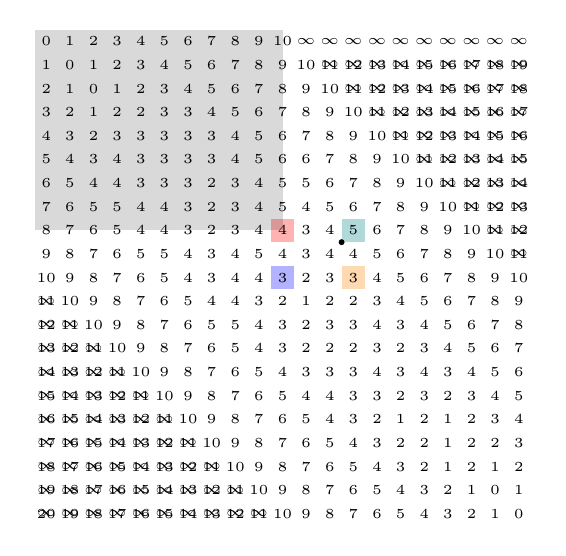
\begin{tikzpicture}[xscale=0.3, yscale=-0.3]

        \fill<3,8->[blue!30] (9.5,9.5) rectangle (10.5, 10.5);
        \fill<4,6->[teal!30] (12.5,7.5) rectangle (13.5, 8.5);

        \fill<10->[orange!30] (12.5,9.5) rectangle (13.5, 10.5);
        \fill<10->[red!30] (9.5,7.5) rectangle (10.5, 8.5);

        \bigpicture{\draw (0, 0) node {\tiny $0$};
\draw (1, 0) node {\tiny $1$};
\draw (2, 0) node {\tiny $2$};
\draw (3, 0) node {\tiny $3$};
\draw (4, 0) node {\tiny $4$};
\draw (5, 0) node {\tiny $5$};
\draw (6, 0) node {\tiny $6$};
\draw (7, 0) node {\tiny $7$};
\draw (8, 0) node {\tiny $8$};
\draw (9, 0) node {\tiny $9$};
\draw (10, 0) node {\tiny $10$};
\draw (11, 0) node {\tiny $\infty$};
\draw (12, 0) node {\tiny $\infty$};
\draw (13, 0) node {\tiny $\infty$};
\draw (14, 0) node {\tiny $\infty$};
\draw (15, 0) node {\tiny $\infty$};
\draw (16, 0) node {\tiny $\infty$};
\draw (17, 0) node {\tiny $\infty$};
\draw (18, 0) node {\tiny $\infty$};
\draw (19, 0) node {\tiny $\infty$};
\draw (20, 0) node {\tiny $\infty$};
\draw (0, 1) node {\tiny $1$};
\draw (1, 1) node {\tiny $0$};
\draw (2, 1) node {\tiny $1$};
\draw (3, 1) node {\tiny $2$};
\draw (4, 1) node {\tiny $3$};
\draw (5, 1) node {\tiny $4$};
\draw (6, 1) node {\tiny $5$};
\draw (7, 1) node {\tiny $6$};
\draw (8, 1) node {\tiny $7$};
\draw (9, 1) node {\tiny $8$};
\draw (10, 1) node {\tiny $9$};
\draw (11, 1) node {\tiny $10$};
\draw (12, 1) node {\tiny $\infty$};
\draw<30-> (12, 1) node {\tiny $11$};
\draw (13, 1) node {\tiny $\infty$};
\draw<30-> (13, 1) node {\tiny $12$};
\draw (14, 1) node {\tiny $\infty$};
\draw<30-> (14, 1) node {\tiny $13$};
\draw (15, 1) node {\tiny $\infty$};
\draw<30-> (15, 1) node {\tiny $14$};
\draw (16, 1) node {\tiny $\infty$};
\draw<30-> (16, 1) node {\tiny $15$};
\draw (17, 1) node {\tiny $\infty$};
\draw<30-> (17, 1) node {\tiny $16$};
\draw (18, 1) node {\tiny $\infty$};
\draw<30-> (18, 1) node {\tiny $17$};
\draw (19, 1) node {\tiny $\infty$};
\draw<30-> (19, 1) node {\tiny $18$};
\draw (20, 1) node {\tiny $\infty$};
\draw<30-> (20, 1) node {\tiny $19$};
\draw (0, 2) node {\tiny $2$};
\draw (1, 2) node {\tiny $1$};
\draw (2, 2) node {\tiny $0$};
\draw (3, 2) node {\tiny $1$};
\draw (4, 2) node {\tiny $2$};
\draw (5, 2) node {\tiny $3$};
\draw (6, 2) node {\tiny $4$};
\draw (7, 2) node {\tiny $5$};
\draw (8, 2) node {\tiny $6$};
\draw (9, 2) node {\tiny $7$};
\draw (10, 2) node {\tiny $8$};
\draw (11, 2) node {\tiny $9$};
\draw (12, 2) node {\tiny $10$};
\draw (13, 2) node {\tiny $\infty$};
\draw<30-> (13, 2) node {\tiny $11$};
\draw (14, 2) node {\tiny $\infty$};
\draw<30-> (14, 2) node {\tiny $12$};
\draw (15, 2) node {\tiny $\infty$};
\draw<30-> (15, 2) node {\tiny $13$};
\draw (16, 2) node {\tiny $\infty$};
\draw<30-> (16, 2) node {\tiny $14$};
\draw (17, 2) node {\tiny $\infty$};
\draw<30-> (17, 2) node {\tiny $15$};
\draw (18, 2) node {\tiny $\infty$};
\draw<30-> (18, 2) node {\tiny $16$};
\draw (19, 2) node {\tiny $\infty$};
\draw<30-> (19, 2) node {\tiny $17$};
\draw (20, 2) node {\tiny $\infty$};
\draw<30-> (20, 2) node {\tiny $18$};
\draw (0, 3) node {\tiny $3$};
\draw (1, 3) node {\tiny $2$};
\draw (2, 3) node {\tiny $1$};
\draw (3, 3) node {\tiny $2$};
\draw (4, 3) node {\tiny $2$};
\draw (5, 3) node {\tiny $3$};
\draw (6, 3) node {\tiny $3$};
\draw (7, 3) node {\tiny $4$};
\draw (8, 3) node {\tiny $5$};
\draw (9, 3) node {\tiny $6$};
\draw (10, 3) node {\tiny $7$};
\draw (11, 3) node {\tiny $8$};
\draw (12, 3) node {\tiny $9$};
\draw (13, 3) node {\tiny $10$};
\draw (14, 3) node {\tiny $\infty$};
\draw<30-> (14, 3) node {\tiny $11$};
\draw (15, 3) node {\tiny $\infty$};
\draw<30-> (15, 3) node {\tiny $12$};
\draw (16, 3) node {\tiny $\infty$};
\draw<30-> (16, 3) node {\tiny $13$};
\draw (17, 3) node {\tiny $\infty$};
\draw<30-> (17, 3) node {\tiny $14$};
\draw (18, 3) node {\tiny $\infty$};
\draw<30-> (18, 3) node {\tiny $15$};
\draw (19, 3) node {\tiny $\infty$};
\draw<30-> (19, 3) node {\tiny $16$};
\draw (20, 3) node {\tiny $\infty$};
\draw<30-> (20, 3) node {\tiny $17$};
\draw (0, 4) node {\tiny $4$};
\draw (1, 4) node {\tiny $3$};
\draw (2, 4) node {\tiny $2$};
\draw (3, 4) node {\tiny $3$};
\draw (4, 4) node {\tiny $3$};
\draw (5, 4) node {\tiny $3$};
\draw (6, 4) node {\tiny $3$};
\draw (7, 4) node {\tiny $3$};
\draw (8, 4) node {\tiny $4$};
\draw (9, 4) node {\tiny $5$};
\draw (10, 4) node {\tiny $6$};
\draw (11, 4) node {\tiny $7$};
\draw (12, 4) node {\tiny $8$};
\draw (13, 4) node {\tiny $9$};
\draw (14, 4) node {\tiny $10$};
\draw (15, 4) node {\tiny $\infty$};
\draw<30-> (15, 4) node {\tiny $11$};
\draw (16, 4) node {\tiny $\infty$};
\draw<30-> (16, 4) node {\tiny $12$};
\draw (17, 4) node {\tiny $\infty$};
\draw<30-> (17, 4) node {\tiny $13$};
\draw (18, 4) node {\tiny $\infty$};
\draw<30-> (18, 4) node {\tiny $14$};
\draw (19, 4) node {\tiny $\infty$};
\draw<30-> (19, 4) node {\tiny $15$};
\draw (20, 4) node {\tiny $\infty$};
\draw<30-> (20, 4) node {\tiny $16$};
\draw (0, 5) node {\tiny $5$};
\draw (1, 5) node {\tiny $4$};
\draw (2, 5) node {\tiny $3$};
\draw (3, 5) node {\tiny $4$};
\draw (4, 5) node {\tiny $3$};
\draw (5, 5) node {\tiny $3$};
\draw (6, 5) node {\tiny $3$};
\draw (7, 5) node {\tiny $3$};
\draw (8, 5) node {\tiny $4$};
\draw (9, 5) node {\tiny $5$};
\draw (10, 5) node {\tiny $6$};
\draw (11, 5) node {\tiny $6$};
\draw (12, 5) node {\tiny $7$};
\draw (13, 5) node {\tiny $8$};
\draw (14, 5) node {\tiny $9$};
\draw (15, 5) node {\tiny $10$};
\draw (16, 5) node {\tiny $\infty$};
\draw<30-> (16, 5) node {\tiny $11$};
\draw (17, 5) node {\tiny $\infty$};
\draw<30-> (17, 5) node {\tiny $12$};
\draw (18, 5) node {\tiny $\infty$};
\draw<30-> (18, 5) node {\tiny $13$};
\draw (19, 5) node {\tiny $\infty$};
\draw<30-> (19, 5) node {\tiny $14$};
\draw (20, 5) node {\tiny $\infty$};
\draw<30-> (20, 5) node {\tiny $15$};
\draw (0, 6) node {\tiny $6$};
\draw (1, 6) node {\tiny $5$};
\draw (2, 6) node {\tiny $4$};
\draw (3, 6) node {\tiny $4$};
\draw (4, 6) node {\tiny $3$};
\draw (5, 6) node {\tiny $3$};
\draw (6, 6) node {\tiny $3$};
\draw (7, 6) node {\tiny $2$};
\draw (8, 6) node {\tiny $3$};
\draw (9, 6) node {\tiny $4$};
\draw (10, 6) node {\tiny $5$};
\draw (11, 6) node {\tiny $5$};
\draw (12, 6) node {\tiny $6$};
\draw (13, 6) node {\tiny $7$};
\draw (14, 6) node {\tiny $8$};
\draw (15, 6) node {\tiny $9$};
\draw (16, 6) node {\tiny $10$};
\draw (17, 6) node {\tiny $\infty$};
\draw<30-> (17, 6) node {\tiny $11$};
\draw (18, 6) node {\tiny $\infty$};
\draw<30-> (18, 6) node {\tiny $12$};
\draw (19, 6) node {\tiny $\infty$};
\draw<30-> (19, 6) node {\tiny $13$};
\draw (20, 6) node {\tiny $\infty$};
\draw<30-> (20, 6) node {\tiny $14$};
\draw (0, 7) node {\tiny $7$};
\draw (1, 7) node {\tiny $6$};
\draw (2, 7) node {\tiny $5$};
\draw (3, 7) node {\tiny $5$};
\draw (4, 7) node {\tiny $4$};
\draw (5, 7) node {\tiny $4$};
\draw (6, 7) node {\tiny $3$};
\draw (7, 7) node {\tiny $2$};
\draw (8, 7) node {\tiny $3$};
\draw (9, 7) node {\tiny $4$};
\draw (10, 7) node {\tiny $5$};
\draw (11, 7) node {\tiny $4$};
\draw (12, 7) node {\tiny $5$};
\draw (13, 7) node {\tiny $6$};
\draw (14, 7) node {\tiny $7$};
\draw (15, 7) node {\tiny $8$};
\draw (16, 7) node {\tiny $9$};
\draw (17, 7) node {\tiny $10$};
\draw (18, 7) node {\tiny $\infty$};
\draw<30-> (18, 7) node {\tiny $11$};
\draw (19, 7) node {\tiny $\infty$};
\draw<30-> (19, 7) node {\tiny $12$};
\draw (20, 7) node {\tiny $\infty$};
\draw<30-> (20, 7) node {\tiny $13$};
\draw (0, 8) node {\tiny $8$};
\draw (1, 8) node {\tiny $7$};
\draw (2, 8) node {\tiny $6$};
\draw (3, 8) node {\tiny $5$};
\draw (4, 8) node {\tiny $4$};
\draw (5, 8) node {\tiny $4$};
\draw (6, 8) node {\tiny $3$};
\draw (7, 8) node {\tiny $2$};
\draw (8, 8) node {\tiny $3$};
\draw (9, 8) node {\tiny $4$};
\draw (10, 8) node {\tiny $4$};
\draw (11, 8) node {\tiny $3$};
\draw (12, 8) node {\tiny $4$};
\draw (13, 8) node {\tiny $5$};
\draw (14, 8) node {\tiny $6$};
\draw (15, 8) node {\tiny $7$};
\draw (16, 8) node {\tiny $8$};
\draw (17, 8) node {\tiny $9$};
\draw (18, 8) node {\tiny $10$};
\draw (19, 8) node {\tiny $\infty$};
\draw<30-> (19, 8) node {\tiny $11$};
\draw (20, 8) node {\tiny $\infty$};
\draw<30-> (20, 8) node {\tiny $12$};
\draw (0, 9) node {\tiny $9$};
\draw (1, 9) node {\tiny $8$};
\draw (2, 9) node {\tiny $7$};
\draw (3, 9) node {\tiny $6$};
\draw (4, 9) node {\tiny $5$};
\draw (5, 9) node {\tiny $5$};
\draw (6, 9) node {\tiny $4$};
\draw (7, 9) node {\tiny $3$};
\draw (8, 9) node {\tiny $4$};
\draw (9, 9) node {\tiny $5$};
\draw (10, 9) node {\tiny $4$};
\draw (11, 9) node {\tiny $3$};
\draw (12, 9) node {\tiny $4$};
\draw (13, 9) node {\tiny $4$};
\draw (14, 9) node {\tiny $5$};
\draw (15, 9) node {\tiny $6$};
\draw (16, 9) node {\tiny $7$};
\draw (17, 9) node {\tiny $8$};
\draw (18, 9) node {\tiny $9$};
\draw (19, 9) node {\tiny $10$};
\draw (20, 9) node {\tiny $\infty$};
\draw<30-> (20, 9) node {\tiny $11$};
\draw (0, 10) node {\tiny $10$};
\draw (1, 10) node {\tiny $9$};
\draw (2, 10) node {\tiny $8$};
\draw (3, 10) node {\tiny $7$};
\draw (4, 10) node {\tiny $6$};
\draw (5, 10) node {\tiny $5$};
\draw (6, 10) node {\tiny $4$};
\draw (7, 10) node {\tiny $3$};
\draw (8, 10) node {\tiny $4$};
\draw (9, 10) node {\tiny $4$};
\draw (10, 10) node {\tiny $3$};
\draw (11, 10) node {\tiny $2$};
\draw (12, 10) node {\tiny $3$};
\draw (13, 10) node {\tiny $3$};
\draw (14, 10) node {\tiny $4$};
\draw (15, 10) node {\tiny $5$};
\draw (16, 10) node {\tiny $6$};
\draw (17, 10) node {\tiny $7$};
\draw (18, 10) node {\tiny $8$};
\draw (19, 10) node {\tiny $9$};
\draw (20, 10) node {\tiny $10$};
\draw (0, 11) node {\tiny $\infty$};
\draw<30-> (0, 11) node {\tiny $11$};
\draw (1, 11) node {\tiny $10$};
\draw (2, 11) node {\tiny $9$};
\draw (3, 11) node {\tiny $8$};
\draw (4, 11) node {\tiny $7$};
\draw (5, 11) node {\tiny $6$};
\draw (6, 11) node {\tiny $5$};
\draw (7, 11) node {\tiny $4$};
\draw (8, 11) node {\tiny $4$};
\draw (9, 11) node {\tiny $3$};
\draw (10, 11) node {\tiny $2$};
\draw (11, 11) node {\tiny $1$};
\draw (12, 11) node {\tiny $2$};
\draw (13, 11) node {\tiny $2$};
\draw (14, 11) node {\tiny $3$};
\draw (15, 11) node {\tiny $4$};
\draw (16, 11) node {\tiny $5$};
\draw (17, 11) node {\tiny $6$};
\draw (18, 11) node {\tiny $7$};
\draw (19, 11) node {\tiny $8$};
\draw (20, 11) node {\tiny $9$};
\draw (0, 12) node {\tiny $\infty$};
\draw<30-> (0, 12) node {\tiny $12$};
\draw (1, 12) node {\tiny $\infty$};
\draw<30-> (1, 12) node {\tiny $11$};
\draw (2, 12) node {\tiny $10$};
\draw (3, 12) node {\tiny $9$};
\draw (4, 12) node {\tiny $8$};
\draw (5, 12) node {\tiny $7$};
\draw (6, 12) node {\tiny $6$};
\draw (7, 12) node {\tiny $5$};
\draw (8, 12) node {\tiny $5$};
\draw (9, 12) node {\tiny $4$};
\draw (10, 12) node {\tiny $3$};
\draw (11, 12) node {\tiny $2$};
\draw (12, 12) node {\tiny $3$};
\draw (13, 12) node {\tiny $3$};
\draw (14, 12) node {\tiny $4$};
\draw (15, 12) node {\tiny $3$};
\draw (16, 12) node {\tiny $4$};
\draw (17, 12) node {\tiny $5$};
\draw (18, 12) node {\tiny $6$};
\draw (19, 12) node {\tiny $7$};
\draw (20, 12) node {\tiny $8$};
\draw (0, 13) node {\tiny $\infty$};
\draw<30-> (0, 13) node {\tiny $13$};
\draw (1, 13) node {\tiny $\infty$};
\draw<30-> (1, 13) node {\tiny $12$};
\draw (2, 13) node {\tiny $\infty$};
\draw<30-> (2, 13) node {\tiny $11$};
\draw (3, 13) node {\tiny $10$};
\draw (4, 13) node {\tiny $9$};
\draw (5, 13) node {\tiny $8$};
\draw (6, 13) node {\tiny $7$};
\draw (7, 13) node {\tiny $6$};
\draw (8, 13) node {\tiny $5$};
\draw (9, 13) node {\tiny $4$};
\draw (10, 13) node {\tiny $3$};
\draw (11, 13) node {\tiny $2$};
\draw (12, 13) node {\tiny $2$};
\draw (13, 13) node {\tiny $2$};
\draw (14, 13) node {\tiny $3$};
\draw (15, 13) node {\tiny $2$};
\draw (16, 13) node {\tiny $3$};
\draw (17, 13) node {\tiny $4$};
\draw (18, 13) node {\tiny $5$};
\draw (19, 13) node {\tiny $6$};
\draw (20, 13) node {\tiny $7$};
\draw (0, 14) node {\tiny $\infty$};
\draw<30-> (0, 14) node {\tiny $14$};
\draw (1, 14) node {\tiny $\infty$};
\draw<30-> (1, 14) node {\tiny $13$};
\draw (2, 14) node {\tiny $\infty$};
\draw<30-> (2, 14) node {\tiny $12$};
\draw (3, 14) node {\tiny $\infty$};
\draw<30-> (3, 14) node {\tiny $11$};
\draw (4, 14) node {\tiny $10$};
\draw (5, 14) node {\tiny $9$};
\draw (6, 14) node {\tiny $8$};
\draw (7, 14) node {\tiny $7$};
\draw (8, 14) node {\tiny $6$};
\draw (9, 14) node {\tiny $5$};
\draw (10, 14) node {\tiny $4$};
\draw (11, 14) node {\tiny $3$};
\draw (12, 14) node {\tiny $3$};
\draw (13, 14) node {\tiny $3$};
\draw (14, 14) node {\tiny $4$};
\draw (15, 14) node {\tiny $3$};
\draw (16, 14) node {\tiny $4$};
\draw (17, 14) node {\tiny $3$};
\draw (18, 14) node {\tiny $4$};
\draw (19, 14) node {\tiny $5$};
\draw (20, 14) node {\tiny $6$};
\draw (0, 15) node {\tiny $\infty$};
\draw<30-> (0, 15) node {\tiny $15$};
\draw (1, 15) node {\tiny $\infty$};
\draw<30-> (1, 15) node {\tiny $14$};
\draw (2, 15) node {\tiny $\infty$};
\draw<30-> (2, 15) node {\tiny $13$};
\draw (3, 15) node {\tiny $\infty$};
\draw<30-> (3, 15) node {\tiny $12$};
\draw (4, 15) node {\tiny $\infty$};
\draw<30-> (4, 15) node {\tiny $11$};
\draw (5, 15) node {\tiny $10$};
\draw (6, 15) node {\tiny $9$};
\draw (7, 15) node {\tiny $8$};
\draw (8, 15) node {\tiny $7$};
\draw (9, 15) node {\tiny $6$};
\draw (10, 15) node {\tiny $5$};
\draw (11, 15) node {\tiny $4$};
\draw (12, 15) node {\tiny $4$};
\draw (13, 15) node {\tiny $3$};
\draw (14, 15) node {\tiny $3$};
\draw (15, 15) node {\tiny $2$};
\draw (16, 15) node {\tiny $3$};
\draw (17, 15) node {\tiny $2$};
\draw (18, 15) node {\tiny $3$};
\draw (19, 15) node {\tiny $4$};
\draw (20, 15) node {\tiny $5$};
\draw (0, 16) node {\tiny $\infty$};
\draw<30-> (0, 16) node {\tiny $16$};
\draw (1, 16) node {\tiny $\infty$};
\draw<30-> (1, 16) node {\tiny $15$};
\draw (2, 16) node {\tiny $\infty$};
\draw<30-> (2, 16) node {\tiny $14$};
\draw (3, 16) node {\tiny $\infty$};
\draw<30-> (3, 16) node {\tiny $13$};
\draw (4, 16) node {\tiny $\infty$};
\draw<30-> (4, 16) node {\tiny $12$};
\draw (5, 16) node {\tiny $\infty$};
\draw<30-> (5, 16) node {\tiny $11$};
\draw (6, 16) node {\tiny $10$};
\draw (7, 16) node {\tiny $9$};
\draw (8, 16) node {\tiny $8$};
\draw (9, 16) node {\tiny $7$};
\draw (10, 16) node {\tiny $6$};
\draw (11, 16) node {\tiny $5$};
\draw (12, 16) node {\tiny $4$};
\draw (13, 16) node {\tiny $3$};
\draw (14, 16) node {\tiny $2$};
\draw (15, 16) node {\tiny $1$};
\draw (16, 16) node {\tiny $2$};
\draw (17, 16) node {\tiny $1$};
\draw (18, 16) node {\tiny $2$};
\draw (19, 16) node {\tiny $3$};
\draw (20, 16) node {\tiny $4$};
\draw (0, 17) node {\tiny $\infty$};
\draw<30-> (0, 17) node {\tiny $17$};
\draw (1, 17) node {\tiny $\infty$};
\draw<30-> (1, 17) node {\tiny $16$};
\draw (2, 17) node {\tiny $\infty$};
\draw<30-> (2, 17) node {\tiny $15$};
\draw (3, 17) node {\tiny $\infty$};
\draw<30-> (3, 17) node {\tiny $14$};
\draw (4, 17) node {\tiny $\infty$};
\draw<30-> (4, 17) node {\tiny $13$};
\draw (5, 17) node {\tiny $\infty$};
\draw<30-> (5, 17) node {\tiny $12$};
\draw (6, 17) node {\tiny $\infty$};
\draw<30-> (6, 17) node {\tiny $11$};
\draw (7, 17) node {\tiny $10$};
\draw (8, 17) node {\tiny $9$};
\draw (9, 17) node {\tiny $8$};
\draw (10, 17) node {\tiny $7$};
\draw (11, 17) node {\tiny $6$};
\draw (12, 17) node {\tiny $5$};
\draw (13, 17) node {\tiny $4$};
\draw (14, 17) node {\tiny $3$};
\draw (15, 17) node {\tiny $2$};
\draw (16, 17) node {\tiny $2$};
\draw (17, 17) node {\tiny $1$};
\draw (18, 17) node {\tiny $2$};
\draw (19, 17) node {\tiny $2$};
\draw (20, 17) node {\tiny $3$};
\draw (0, 18) node {\tiny $\infty$};
\draw<30-> (0, 18) node {\tiny $18$};
\draw (1, 18) node {\tiny $\infty$};
\draw<30-> (1, 18) node {\tiny $17$};
\draw (2, 18) node {\tiny $\infty$};
\draw<30-> (2, 18) node {\tiny $16$};
\draw (3, 18) node {\tiny $\infty$};
\draw<30-> (3, 18) node {\tiny $15$};
\draw (4, 18) node {\tiny $\infty$};
\draw<30-> (4, 18) node {\tiny $14$};
\draw (5, 18) node {\tiny $\infty$};
\draw<30-> (5, 18) node {\tiny $13$};
\draw (6, 18) node {\tiny $\infty$};
\draw<30-> (6, 18) node {\tiny $12$};
\draw (7, 18) node {\tiny $\infty$};
\draw<30-> (7, 18) node {\tiny $11$};
\draw (8, 18) node {\tiny $10$};
\draw (9, 18) node {\tiny $9$};
\draw (10, 18) node {\tiny $8$};
\draw (11, 18) node {\tiny $7$};
\draw (12, 18) node {\tiny $6$};
\draw (13, 18) node {\tiny $5$};
\draw (14, 18) node {\tiny $4$};
\draw (15, 18) node {\tiny $3$};
\draw (16, 18) node {\tiny $2$};
\draw (17, 18) node {\tiny $1$};
\draw (18, 18) node {\tiny $2$};
\draw (19, 18) node {\tiny $1$};
\draw (20, 18) node {\tiny $2$};
\draw (0, 19) node {\tiny $\infty$};
\draw<30-> (0, 19) node {\tiny $19$};
\draw (1, 19) node {\tiny $\infty$};
\draw<30-> (1, 19) node {\tiny $18$};
\draw (2, 19) node {\tiny $\infty$};
\draw<30-> (2, 19) node {\tiny $17$};
\draw (3, 19) node {\tiny $\infty$};
\draw<30-> (3, 19) node {\tiny $16$};
\draw (4, 19) node {\tiny $\infty$};
\draw<30-> (4, 19) node {\tiny $15$};
\draw (5, 19) node {\tiny $\infty$};
\draw<30-> (5, 19) node {\tiny $14$};
\draw (6, 19) node {\tiny $\infty$};
\draw<30-> (6, 19) node {\tiny $13$};
\draw (7, 19) node {\tiny $\infty$};
\draw<30-> (7, 19) node {\tiny $12$};
\draw (8, 19) node {\tiny $\infty$};
\draw<30-> (8, 19) node {\tiny $11$};
\draw (9, 19) node {\tiny $10$};
\draw (10, 19) node {\tiny $9$};
\draw (11, 19) node {\tiny $8$};
\draw (12, 19) node {\tiny $7$};
\draw (13, 19) node {\tiny $6$};
\draw (14, 19) node {\tiny $5$};
\draw (15, 19) node {\tiny $4$};
\draw (16, 19) node {\tiny $3$};
\draw (17, 19) node {\tiny $2$};
\draw (18, 19) node {\tiny $1$};
\draw (19, 19) node {\tiny $0$};
\draw (20, 19) node {\tiny $1$};
\draw (0, 20) node {\tiny $\infty$};
\draw<30-> (0, 20) node {\tiny $20$};
\draw (1, 20) node {\tiny $\infty$};
\draw<30-> (1, 20) node {\tiny $19$};
\draw (2, 20) node {\tiny $\infty$};
\draw<30-> (2, 20) node {\tiny $18$};
\draw (3, 20) node {\tiny $\infty$};
\draw<30-> (3, 20) node {\tiny $17$};
\draw (4, 20) node {\tiny $\infty$};
\draw<30-> (4, 20) node {\tiny $16$};
\draw (5, 20) node {\tiny $\infty$};
\draw<30-> (5, 20) node {\tiny $15$};
\draw (6, 20) node {\tiny $\infty$};
\draw<30-> (6, 20) node {\tiny $14$};
\draw (7, 20) node {\tiny $\infty$};
\draw<30-> (7, 20) node {\tiny $13$};
\draw (8, 20) node {\tiny $\infty$};
\draw<30-> (8, 20) node {\tiny $12$};
\draw (9, 20) node {\tiny $\infty$};
\draw<30-> (9, 20) node {\tiny $11$};
\draw (10, 20) node {\tiny $10$};
\draw (11, 20) node {\tiny $9$};
\draw (12, 20) node {\tiny $8$};
\draw (13, 20) node {\tiny $7$};
\draw (14, 20) node {\tiny $6$};
\draw (15, 20) node {\tiny $5$};
\draw (16, 20) node {\tiny $4$};
\draw (17, 20) node {\tiny $3$};
\draw (18, 20) node {\tiny $2$};
\draw (19, 20) node {\tiny $1$};
\draw (20, 20) node {\tiny $0$};

}

        \filldraw<12> (12.5,8.5) circle(0.1);

        \fill<14>[opacity=0.15] (-0.5,-0.5) rectangle (10,8);

        \end{tikzpicture}
    \end{center}
  \end{column}%
\end{columns}%

\end{frame}


\begin{frame}{Core-Sparse Monge Matrices}
  \begin{alertblock}{Monge Matrix}
    A matrix $M\in \mathbb{R}^{n\times m}$ is a \textbf{Monge} matrix if, for every $i\in [0\dd n-1)$ and $j\in [0\dd m-1)$,
    
    {\hfill  $M^{\square}[i,j]:=M[i+1,j]+M[i,j+1]-M[i+1,j+1]-M[i,j]\ge 0.$\hfill \;}
  \end{alertblock}
  \pause
    \[M[i,j] = M[i,0] + M[0,j] - M[0][0] - \sum_{i'=0}^{i-1}\sum_{j'=0}^{j-1} M^\square[i',j']\]
  \pause 
  \begin{fact}[Core-Sparse Representation {[Wil85]}]
    If $M\in \mathbb{R}^{n\times m}$ and $M^\square$ has $c$ non-zero entries, then $M$ can be stored in $\Oh(n+m+c\log c)$ space so that $M[i,j]$ can be computed in $\Oh(\log c)$ time.
  \end{fact}

  \pause\medskip
  \textbf{Observation:}
  $D_{X,Y}\in \mathbb{Z}_{\ge 0}^{(|X|+|Y|+1)\times (|X|+|Y|+1)}$ is Monge, and its core size is $\le 2(|X|+|Y|)$.

\end{frame}


\begin{frame}{Min-Plus Product of Core-Sparse Monge Matrices}

  \begin{fact}[{[SMAWK87]}]
    If $A,B\in \mathbb{R}^{n\times n}$ are Monge matrices, then $A\otimes B$ can be constructed in $\Oh(n^2)$ time.
  \end{fact}

  \bigskip
  \pause

  \begin{fact}[{[Tis08,Rus10,GG\textbf{K}24]}]
    If $A,B\in \mathbb{R}^{n\times n}$ are Monge matrices and $A$, $B$, and $A\otimes B$ all have cores of size at most $c$, then $A\otimes B$ can be constructed in $\Ohtilde(n+c)$ time.
  \end{fact}
  \bigskip
  \pause
  \begin{alertblock}{Theorem ([C\textbf{K}M20])}
    The core of the distance matrix $D_{X,Y}$ can be maintained in $\Ohtilde(n)$ time per update (character edit) in $X,Y\in \Sigma^{\le n}$. 
   \end{alertblock}

\end{frame}


\begin{frame}{Substitutions Only}
    \begin{columns}
        \begin{column}{0.5\textwidth}
            \begin{itemize}
                \item<1-> The optimal path stays within a band of width $\Oh(k)$.
                \item<2-> Cover the band with $\Oh(\frac{n}{k})$ boxes of size $\Oh(k)\times \Oh(k)$.
                \item<3-> Optimal path crosses each $V_i$.
                \item<4-> $D_{i, j}$: the matrix of distances $V_i\leadsto V_j$.
                \item<5-> $\tOh(k^2 \cdot \frac{n}{k}) = \tOh(nk)$ time for initializing distance matrices of all boxes.
                \item<5-> $\tOh(k)$ time per update for recomputing the distance matrices of affected boxes.
            \end{itemize}
        \end{column}
        \begin{column}{0.5\textwidth}
            \begin{center}
            \begin{tikzpicture}[transform canvas={scale=0.55}, y=-1cm, xshift=-5.3cm, yshift=6cm]
                \bigpicture{
\def\shft{0}
\def\W{12}
\def\H{12}
\def\myi{2}
\def\cnt{6}
\def\gp{2}
\def\kp{1.5}
\def\charwidth{1 / 15}
%\draw[black,thin] (-1,-1) grid (\H + 1,\W + 1);

%0/gray,1/red,2/violet,3/blue,4/magenta,5/orange,6/green,7/yellow

\foreach \x/\c/\d/\e in {0/gray/darkblue/gray,\gp/violet/darkblue/darkblue,2*\gp/orange/purple/purple,3*\gp/magenta/purple/purple,4*\gp/yellow/purple/purple,5*\gp/yellow/purple/yellow} {
    \draw<2-4>[fill=\c!40,thick] (\x, {max(\x - \kp, 0)}) rectangle (\x + \gp, {min(\x + \gp + \kp, \H)});
    \draw<5->[fill=\e!40, thick] (\x, {max(\x - \kp, 0)}) rectangle (\x + \gp, {min(\x + \gp + \kp, \H)});
    \draw<8->[densely dotted,step=0.5cm] (\x, {max(\x - \kp, 0)}) grid (\x + \gp, {min(\x + \gp + \kp, \H)});
}

\onslide<9>{
  \foreach \y in {0,.5,...,3} {
      \foreach \x in {0,0.5,...,1.5} {
        \pgfmathrandominteger{\r}{0}{3}
      % map 0..3 to the four colors
        \ifcase\r\relax
        \def\cellcolor{gray}%
        \or
        \def\cellcolor{darkblue}%
        \or
        \def\cellcolor{purple}%
        \or
        \def\cellcolor{yellow}%
        \fi
          \path[fill=\cellcolor!40] (\x,\y) rectangle ++(.5,.5); 
      }
  }
    \foreach \y in {0,0.5,...,4.5} {
      \foreach \x in {0,0.5,...,1.5} {
        \pgfmathrandominteger{\r}{0}{3}
      % map 0..3 to the four colors
        \ifcase\r\relax
        \def\cellcolor{gray}%
        \or
        \def\cellcolor{darkblue}%
        \or
        \def\cellcolor{purple}%
        \or
        \def\cellcolor{yellow}%
        \fi
          \path[fill=\cellcolor!40] (2+\x,.5+\y) rectangle ++(.5,.5); 
      }
  }
      \foreach \y in {0,0.5,...,4.5} {
      \foreach \x in {0,0.5,...,1.5} {
        \pgfmathrandominteger{\r}{0}{3}
      % map 0..3 to the four colors
        \ifcase\r\relax
        \def\cellcolor{gray}%
        \or
        \def\cellcolor{darkblue}%
        \or
        \def\cellcolor{purple}%
        \or
        \def\cellcolor{yellow}%
        \fi
          \path[fill=\cellcolor!40] (4+\x,2.5+\y) rectangle ++(.5,.5); 
          \path[fill=\cellcolor!40] (6+\x,4.5+\y) rectangle ++(.5,.5); 
          \path[fill=\cellcolor!40] (8+\x,6.5+\y) rectangle ++(.5,.5); 

      }
  }

    \foreach \y in {8.5,9,...,11.5} {
      \foreach \x in {10,10.5,...,11.5} {
        \pgfmathrandominteger{\r}{0}{3}
      % map 0..3 to the four colors
        \ifcase\r\relax
        \def\cellcolor{gray}%
        \or
        \def\cellcolor{darkblue}%
        \or
        \def\cellcolor{purple}%
        \or
        \def\cellcolor{yellow}%
        \fi
          \path[fill=\cellcolor!40] (\x,\y) rectangle ++(.5,.5); 
      }
  }
}

%\foreach \x/\c in {} {
%    \draw<2-4>[fill=\c!40, thick] (\x, {max(\x - \kp, 0)}) rectangle (\x + \gp, {min(\x + \gp + \kp, \H)});
%    \draw<5->[fill=darkblue!40, thick] (\x, {max(\x - \kp, 0)}) rectangle (\x + \gp, {min(\x + \gp + \kp, \H)});
%}

%\foreach \x in {4*\gp} {
%    \draw<2-5>[fill=darkblue!40, thick] (\x, {max(\x - \kp, 0)}) rectangle (\x + \gp, {min(\x + \gp + \kp, \H)});
%    \draw<6->[fill=darkblue!70, thick] (\x, {max(\x - \kp, 0)}) rectangle (\x + \gp, {min(\x + \gp + \kp, \H)});
%}

\draw (\kp,0.1) -- (\kp,-0.1) node[above] {$k$};
\draw (0.1,\kp) -- (-0.1,\kp) node[left] {$k$};
\draw[fill=darkgreen,fill opacity=0.1] (0, 0) -- (\kp, 0) -- (\H, \W - \kp) -- (\H, \W) -- (\H - \kp, \W) -- (0, \kp) -- (0, 0);

\onslide<2->{
\foreach \x in {0,\gp,...,{\the\numexpr \W - \gp}}
    \draw (\x, {max(\x - \kp, 0)}) rectangle (\x + \gp, {min(\x + \kp + \gp, \H)});
}

\draw[thick] (0, 0) rectangle (\H, \W);

\onslide<2->{
\draw (0,0.1) -- (0,0) node[above] {$x_0$};
\draw (\W,0.1) -- (\W,0) node[above] {$x_{\cnt}$};
\foreach \x in {1,2,...,{\the\numexpr \cnt - 1}}
    \draw (\x * \gp,0.1) -- (\x * \gp, -0.1) node[above] {$x_{\x}$};


\draw[dashed] (\myi * \gp + \gp, 0) -- (\myi * \gp + \gp, \myi * \gp);
\draw[dashed] (0,\myi * \gp - \kp) node[left] {$x_{\myi} - k$} -- (\myi * \gp,\myi * \gp - \kp);
\draw[dashed] (0,\myi * \gp + \gp + \kp) node[left] {$x_{\the\numexpr \myi + 1} + k$} -- (\myi * \gp,\myi * \gp + \kp+ \gp);
}

\node<3->[left, black] at (\myi * \gp, \myi * \gp) {$V_{\myi}$};
\node<3->[right, black] at (\myi * \gp + \gp, \myi * \gp + \gp) {$V_{\the\numexpr \myi + 1}$};

\draw<3->[very thick, darkgreen] (\myi * \gp, \myi * \gp - \kp) -- (\myi * \gp, \myi * \gp + \kp);
\draw<3->[very thick, darkgreen] (\myi * \gp + \gp, \myi * \gp+\gp-\kp) -- (\myi * \gp + \gp, \myi * \gp + \gp + \kp);

%\node<4->[darkred] at (\myi * \gp + \gp / 2, \myi * \gp + \gp / 2) {\Large $D_{\myi, {\the\numexpr \myi + 1}}$};


%\draw<6->[fill=orange, thick,opacity=0.4] (4.2 * \gp - 1.0 * \gp * \charwidth, 0) rectangle (4.2 * \gp + 1.0 * \gp * \charwidth, \H);
%\draw<7->[fill=orange, thick,opacity=0.4] (0, 2.5 * \gp - 1.0 * \gp * \charwidth) rectangle (\W, 2.5 * \gp + 1.0 * \gp * \charwidth);
}
            \end{tikzpicture}
            \end{center}
        \end{column}
    \end{columns}
  \end{frame}

%\ end{comment}
  
  \begin{frame}[fragile]{Substitutions Only}
    \begin{columns}
        \begin{column}{0.5\textwidth}
            \[D_{0,m} = \bigotimes_{i=0}^{m-1} D_{i,i+1}\]
            \begin{itemize}
                \item<2-> $D_{i,j}$'s can be $(\min, +)$-multiplied in $\tOh(k)$ time.
                \item<3-> $\tOh(\frac{n}{k} \cdot k)=\tOh(n)$ time for initializing the tree of $D_{i,j}$ matrices.
                \item<4-> $\tOh(k)$ time per update for maintaining the tree of $D_{i,j}$ matrices.
            \end{itemize}
        \end{column}
        \begin{column}{0.5\textwidth}
            \begin{tikzpicture}[every node/.style = {minimum width = 2em, draw}, level/.style = {sibling distance = 35mm/#1}, edge from parent/.style={draw}]
                \bigpicture{\onslide<-3>{
\node{$D_{0, 6}$} child {
    node{$D_{0, 3}$} child {
        node{$D_{0, 2}$} child {
            node{$D_{0, 1}$}
        } child {
            node{$D_{1, 2}$}
        }
    } child {
        node{$D_{2, 3}$}
    }
} child {
    node{$D_{3, 6}$} child {
        node{$D_{3, 5}$} child {
            node{$D_{3, 4}$}
        } child {
            node{$D_{4, 5}$}
        }
    } child {
        node{$D_{5, 6}$}
    }
};
}

\onslide<4->{
\node[fill=darkblue!50]{$D_{0, 6}$} child {
    node{$D_{0, 3}$} child {
        node{$D_{0, 2}$} child {
            node{$D_{0, 1}$}
        } child {
            node{$D_{1, 2}$}
        }
    } child {
        node{$D_{2, 3}$}
    }
} child {
    node[fill=darkblue!50]{$D_{3, 6}$} child {
        node[fill=darkblue!50]{$D_{3, 5}$} child {
            node{$D_{3, 4}$}
        } child {
            node[fill=darkblue!50]{$D_{4, 5}$}
        }
    } child {
        node{$D_{5, 6}$}
    }
};
}
}
            \end{tikzpicture}
        \end{column}
    \end{columns}
  \end{frame}


  
  \begin{frame}{Supporting Insertions and Deletions: Challenges}
    \begin{columns}
        \begin{column}{0.5\textwidth}
            \begin{itemize}
                \item<1-> Every substitution affects $\Oh(1)$ boxes, but a single insertion may shift \emph{all} boxes.
                \item<7-> After $\Omega(k)$ updates the boxes can be completely disjoint with the stripe.
                %\item<8-> Boxes of size $\Theta(k)\times \Theta(t)$ needed to support $t\ge k$ updates.
                %\item<9-> $\tOh(\frac{n}{k}\cdot kt)=\tOh(nt)$-time initialization amortizes to $\tOh(n)$ per update~--- no improvement over \where{C\textbf{K}M20}.
                \item<8-> $\tOh(nk)$-time initialization amortizes to $\tOh(n)$ per update~--- no improvement over \where{C\textbf{K}M20}.
                \item<12-> Even if update locations are known in advance, $\tOh(k^2)$-time initialization per update is needed~--- no improvement over \where{LV88+MSU94}.
            \end{itemize}
        \end{column}
        \begin{column}{0.5\textwidth}
            \begin{center}
            \begin{tikzpicture}[transform canvas={scale=0.55}, y=-1cm, xshift=-5.3cm, yshift=6cm]
                \bigpicture{
                
\def\shft{0}
\def\W{12}
\def\H{12}
\def\myi{2}
\def\cnt{6}
\def\gp{2}
\def\kp{1}
\def\strlen{12}
\def\charwidth{1 / 15}
%\draw[black,thin] (-1,-1) grid (\H + 1,\W + 1);

 \foreach \iter in {0,1,...,{\the\numexpr 3 * \gp}} {
     \foreach \x in {1,2,...,{\the\numexpr \strlen + 1}} {
        \ifthenelse{\x > \strlen}{
            \ifthenelse{\iter > 0}{
                \fill<{\the\numexpr \iter + 1}>[red!50] (-0.1, \x * \H / \strlen) rectangle (-0.4, \x* \H / \strlen - \H/\strlen);
            }{}
        }{
            \ifthenelse{\(\x < \iter\) \OR \(\x = \iter\)}{
                \fill<{\the\numexpr \iter + 1}>[green!50] (-0.1, \x * \H / \strlen) rectangle (-0.4, \x* \H / \strlen - \H/\strlen);
            }{}
        }
    }
    \draw<{\the\numexpr \iter + 1}> (-0.1, 0) rectangle (-0.4,\H);
    \foreach \x in {0,\gp,...,{\the\numexpr \W - \gp}}
        \draw<{\the\numexpr \iter + 1}>[fill=darkblue!40, thick] (\x, {min(max(\x - \kp + \iter, 0), \H)}) rectangle (\x + \gp, {min(\x + \kp + \gp + \iter, \H)});
}

\foreach \iter in {8,9,...,12} {
    \foreach \x in {0,1,...,{\the\numexpr \cnt - 1}} {
        \ifthenelse{\(\x = 1 \AND \iter > 8\) \OR \(\x = 4 \AND \iter > 9\) \OR \(\x = 3 \AND \iter > 10\) \OR \(\x = 5 \AND \iter > 10\)}{
            \draw<\iter>[fill=darkblue!70, thick] (\x * \gp, {max(\x * \gp - 2*\kp, 0)}) rectangle (\x * \gp + \gp, {min(\x * \gp + \gp + 2*\kp, \H)});
        }{
            \draw<\iter>[fill=darkblue!40, thick] (\x * \gp, {max(\x * \gp - 2*\kp, 0)}) rectangle (\x * \gp + \gp, {min(\x * \gp + \gp + 2*\kp, \H)});
        }
    }
}

\draw[fill=darkgreen!40] (0, 0) -- (\kp, 0) -- (\H, \W - \kp) -- (\H, \W) -- (\H - \kp, \W) -- (0, \kp) -- (0, 0);

\onslide<8->{
\draw[dashed] (0,\myi * \gp - 2*\kp) node[left] {$x_{\myi} - 2k$} -- (\myi * \gp,\myi * \gp - 2*\kp);
\draw[dashed] (0,\myi * \gp + \gp + 2*\kp) node[left] {$x_{\the\numexpr \myi + 1} + 2k$} -- (\myi * \gp,\myi * \gp + 2*\kp+ \gp);
}

\draw<9->[fill=orange, thick,opacity=0.4] (1.5 * \gp - 1.0 * \gp * \charwidth, 0) rectangle (1.5 * \gp + 1.0 * \gp * \charwidth, \H);
\draw<10->[fill=orange, thick,opacity=0.4] (4.2 * \gp - 1.0 * \gp * \charwidth, 0) rectangle (4.2 * \gp + 1.0 * \gp * \charwidth, \H);
\draw<11->[fill=orange, thick,opacity=0.4] (0, 4.7 * \gp - 1.0 * \gp * \charwidth) rectangle (\W, 4.7 * \gp + 1.0 * \gp * \charwidth);

\foreach \iter in {0,1,...,{\the\numexpr 3 * \gp}} {
    \foreach \x in {0,\gp,...,{\the\numexpr \W - \gp}}
        \draw<{\the\numexpr \iter + 1}> (\x, {min(max(\x - \kp + \iter, 0), \H)}) rectangle (\x + \gp, {min(\x + \gp + \kp + \iter, \H)});
}

%\foreach \x in {0,\gp,...,{\the\numexpr \W - \gp}}
%    \draw<8> (\x, {max(\x - \gp, 0)}) rectangle (\x + \gp, {min(\x + \gp + \gp, \H)});

\foreach \iter in {8,9,...,12} {
    \foreach \x in {0,1,...,{\the\numexpr \cnt - 1}} {
        \draw<\iter> (\x * \gp, {max(\x * \gp - 2*\kp, 0)}) rectangle (\x * \gp + \gp, {min(\x * \gp + \gp + 2*\kp, \H)});
    }
}

\draw[thick] (0, 0) rectangle (\H, \W);

\draw (0,0.1) -- (0,0) node[above] {$x_0$};
\draw (\W,0.1) -- (\W,0) node[above] {$x_{\cnt}$};
\foreach \x in {1,2,...,{\the\numexpr \cnt - 1}}
    \draw (\x * \gp,0.1) -- (\x * \gp, -0.1) node[above] {$x_{\x}$};



%\foreach \x in {0,1,...,{\the\numexpr \cnt - 1}} {
%    \draw<9->[thick] (\gp * \x, {max(\gp * \x - \gp, 0)}) -- (\gp * \x + \gp, {max(\gp * \x - \gp, 0)}) -- (\gp * \x + \gp, \gp * \x);
%    \draw<9->[thick] (\gp * \x, {min(\gp * \x + \gp, \H)}) -- (\gp * \x, {min(\gp * \x + 2 * \gp, \H)}) -- (\gp * \x + \gp, {min(\gp * \x + 2 * \gp, \H)});
%}

                }
            \end{tikzpicture}
            \end{center}
            %*Picture of shifting boxes, and specifying which boxes will change and how it affects the way the algorithm could work*
        \end{column}
    \end{columns}
  \end{frame}


    \begin{frame}{Few Distinct Boxes}
    \begin{columns}
        \begin{column}{0.5\textwidth}
            \textbf{Goal:} Achieve $\Ohtilde(k^2)$-time preprocessing.
            \medskip

            \textbf{Assumptions:} 
            \begin{itemize}
               \item $\ed(X,Y)=\Oh(k)$,
               \item $\sed(X)=\Oh(k)$.
            \end{itemize}

            \medskip\pause
            \textbf{Idea:} 
            \begin{itemize}
                \item<2-> Use the decomposition $X=\bigodot_{i=1}^{m}X_i$ from $\sed(X)$.
                \item<9-> Only $\Oh(k)$ boxes are not isomorphic to the previous one.
                \item<10-> Still $\tOh(k^3)$ preprocessing time~--- amortizes to $\tOh(k^2)$ per update.
                \item<11-> Even if $X_i \neq X_{i-1}$, we can hope to reuse some information.
            \end{itemize}
        \end{column}
        \begin{column}{0.5\textwidth}
            \centering
            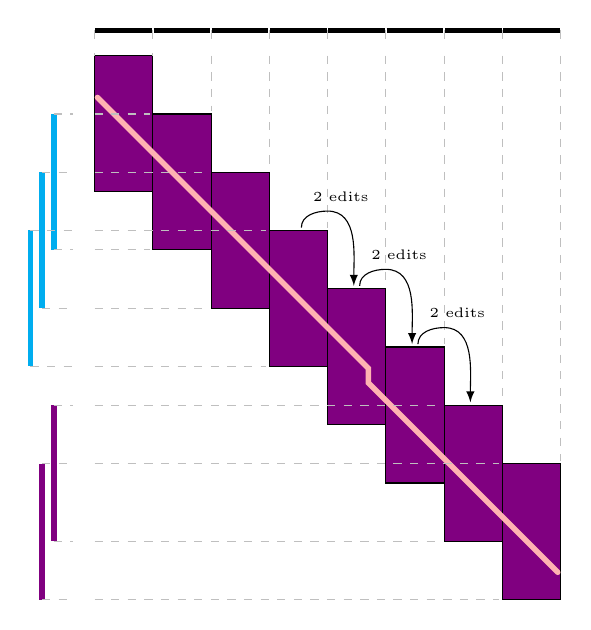
\begin{tikzpicture}[scale=0.37, y=-1cm]
                \bigpicture{
                    
\def\W{16}
\def\H{16}
\def\cnt{7}
\def\gp{2}

\draw<4->[fill=yellow!40] (8, 9.4) rectangle (12, 9.9);

\foreach \iter in {0,1,...,9}
    \foreach \x in {0,1,...,\cnt}
        \ifthenelse{\x > 0 \AND \x < 4 \AND \iter > 3}{
            \draw<{\the \numexpr\iter+2}>[fill=cyan] (\x * \gp, \x * \gp - 2*\gp / 3) rectangle (\x * \gp + \gp, \x * \gp + \gp + 2*\gp / 3);
        }{
            \ifthenelse{\x > 5 \AND \iter > 5}{
                \draw<{\the \numexpr\iter+2}>[fill=violet] (\x * \gp, \x * \gp - 2*\gp / 3) rectangle (\x * \gp + \gp, \x * \gp + \gp + 2*\gp / 3);
            }{
                \draw<{\the \numexpr\iter+2}> (\x * \gp, \x * \gp - 2*\gp / 3) rectangle (\x * \gp + \gp, \x * \gp + \gp + 2*\gp / 3);
            };
        };



\draw<3->[line width=2pt, red!30,line cap=round] (0.1, 0.1) -- (9.4, 9.4) -- (9.4, 9.9) -- (\H - 0.1, \W + 0.4);

\foreach \x in {0,1,...,\cnt}{
    \draw[line width=2pt] (\x * \gp+0.03,-2.2) -- (\x * \gp + \gp-0.03,-2.2);
    \draw[dashed, lightgray] (\x * \gp+\gp, -2*\gp / 3) -- (\x * \gp+\gp, \x * \gp - 2*\gp / 3 - 0.1);
    \draw[dashed, lightgray] (\x * \gp+\gp, -2.2) -- (\x * \gp+\gp, -1.9);
}
\draw[dashed, lightgray] (0, -2*\gp / 3) -- (0, - 2*\gp / 3 - 0.1);
\draw[dashed, lightgray] (0, -2.2) -- (0, -1.9);

\onslide<5->{
\foreach \x in {1,2,3}{
    \draw[cyan,line width=2pt] (-1-0.4*\x,\x * \gp - 2*\gp / 3) -- (-1-0.4*\x,\x * \gp + \gp + 2*\gp / 3);
    \draw[dashed, lightgray] (0, \x * \gp - 2*\gp / 3) -- (\x * \gp - 0.1, \x * \gp - 2*\gp / 3);
    \draw[dashed, lightgray] (-1-0.4*\x, \x * \gp - 2*\gp / 3) -- (-0.75, \x * \gp - 2*\gp / 3);
    \draw[dashed, lightgray] (0, \x * \gp + \gp + 2*\gp / 3) -- (\x * \gp - 0.1, \x * \gp + \gp + 2*\gp / 3);
    \draw[dashed, lightgray] (-1-0.4*\x, \x * \gp + \gp + 2*\gp / 3) -- (-0.75, \x * \gp + \gp + 2*\gp / 3);
}
}

\onslide<7->{

\foreach \x in {6,7}{
    \draw[violet,line width=2pt] (-0.4*\x+1,\x * \gp - 2*\gp / 3) -- (-0.4*\x+1,\x * \gp + \gp + 2*\gp / 3);
    \draw[dashed, lightgray] (0, \x * \gp - 2*\gp / 3) -- (\x * \gp - 0.1, \x * \gp - 2*\gp / 3);
    \draw[dashed, lightgray] (1-0.4*\x, \x * \gp - 2*\gp / 3) -- (-0.75, \x * \gp - 2*\gp / 3);
    \draw[dashed, lightgray] (0, \x * \gp + \gp + 2*\gp / 3) -- (\x * \gp - 0.1, \x * \gp + \gp + 2*\gp / 3);
    \draw[dashed, lightgray] (1-0.4*\x, \x * \gp + \gp + 2*\gp / 3) -- (-0.75, \x * \gp + \gp + 2*\gp / 3);
}
}

\onslide<11>{
    \foreach \x in {3,4,5}
\draw<{\the\numexpr \x-1}->[-latex] (\x * \gp + \gp / 2 + 0.1, \x * \gp - 2*\gp / 3 - 0.1) to [out=90,in=180] (\x * \gp + \gp, \x * \gp - \gp) node[above] {\hphantom{sp}\tiny $2$ edits} to [out=0,in=90] (\x * \gp + \gp + \gp / 2 - 0.1, \x * \gp + 1*\gp / 3 - 0.1) ;
}
                }
            \end{tikzpicture}
        \end{column}
    \end{columns}
  \end{frame}

  \begin{frame}{Relationship between Distinct Boxes}
    \begin{columns}
        \begin{column}{0.5\textwidth}%
            \onslide<2->{%
            \textbf{Recall:} If $\sed(X)\le k$, then $X$ can be decomposed into $\le k$ single characters and $\le k$ fragments with a \emph{previous occurrence} $\le k$ positions earlier.
            }

            \bigskip
            \onslide<17->{
            \textbf{Consequence:}
            \begin{itemize}
                    \item<17-> $X_i, Y_i$ can be constructed from $X_{i - 1}, Y_{i - 1}$ with character appends, copy-pastes, and a prefix removal.
                    %\item<16-> $Y_i$ can be constructed from $Y_{i - 1}$ with character appends, copy-pastes, and a prefix removal.
                    \item<18-> Use weight-balanced SLPs \where{CLLPPSS02}.
                    \item<19-> Time complexity:
                        \begin{itemize}
                            \item<19-> $\tOh(k)$ time per operation, $\Oh(k)$ operations across all distinct boxes.
                            \item<19-> Initialization time: $\tOh(k^2)$.
                            \item<19-> Amortized over $\Theta(k)$ updates: $\tOh(k)$.
                       \end{itemize}
                \end{itemize}
            }
        \end{column}
        \begin{column}{0.5\textwidth}
            \vspace*{-0.4cm}
            \begin{center}
            \begin{tikzpicture}[scale=0.53, y=-1cm]
                \bigpicture{
                    \bigpicture{\draw[thick] (1,1) rectangle (5,9);
\draw[thick] (5,4) rectangle (9,12);

\draw[line width=2] (1.05,0) --node[above]{$X_{i-1}$} (4.95, 0);
\draw[line width=2] (5.05,0) --node[above]{$X_{i}$} (8.95, 0);

\draw<3->[line width=2,darkblue] (3.05, 0.2) -- (5.25,0.2);
\draw<5->[line width=2,darkgreen] (5.25, 0.2) -- (5.75,0.2);
\draw<6->[line width=2,darkred] (5.75, 0.2) -- (6,0.2);
\draw<7->[line width=2,olive] (6, 0.2) -- (6.5,0.2);
\draw<8->[line width=2,darkred] (6.5, 0.2) -- (6.75,0.2);
\draw<9->[line width=2,cyan] (6.75, 0.2) -- (6.95,0.2);


\draw<3->[line width=2,darkblue] (5.05, 0.35) -- (7.25,0.35);
\draw<4->[line width=2,darkred] (7.25, 0.35) -- (7.5,0.35);
\draw<5->[line width=2,darkgreen] (7.5, 0.35) -- (8,0.35);
\draw<7->[line width=2,olive] (8, 0.35) -- (8.5,0.35);
\draw<8->[line width=2,darkred] (8.5, 0.35) -- (8.75,0.35);
\draw<9->[line width=2,cyan] (8.75, 0.35) -- (8.95,0.35);

\draw<2>[ultra thick,opacity=0.5] (1.05,1.05) rectangle (4.95,8.95);
\draw<3>[ultra thick,opacity=0.5] (1.05,1.05) rectangle (7.2,8.95);
\draw<4>[ultra thick,opacity=0.5] (1.05,1.05) rectangle (7.45,8.95);
\draw<5-6>[ultra thick,opacity=0.5] (1.05,1.05) rectangle (7.95,8.95);
\draw<7>[ultra thick,opacity=0.5] (1.05,1.05) rectangle (8.45,8.95);
\draw<8>[ultra thick,opacity=0.5] (1.05,1.05) rectangle (8.7,8.95);
\draw<9>[ultra thick,opacity=0.5] (1.05,1.05) rectangle (8.95,8.95);
\draw<10>[ultra thick,opacity=0.5] (5.05,1.05) rectangle (8.95,8.95);

\draw<11>[ultra thick,opacity=0.5] (5.05,1.05) rectangle (8.95,10.45);
\draw<12>[ultra thick,opacity=0.5] (5.05,1.05) rectangle (8.95,10.7);
\draw<13-14>[ultra thick,opacity=0.5] (5.05,1.05) rectangle (8.95,11.45);
\draw<15>[ultra thick,opacity=0.5] (5.05,1.05) rectangle (8.95,11.95);
\draw<16>[ultra thick,opacity=0.5] (5.05,4.05) rectangle (8.95,11.95);


\draw<11->[line width=2,violet] (0.4,6) -- (0.4,7.5);
\draw<12->[line width=2,darkred] (0.4,7.5) -- (0.4,7.75);
\draw<13->[line width=2,yellow] (0.4,7.75) -- (0.4,8.5);
\draw<14->[line width=2,darkred] (0.4,8.5) -- (0.4,8.75);
\draw<15->[line width=2,orange] (0.4,8.75) -- (0.4,9.25);

\draw<7->[line width=2,olive] (6, 0.2) -- (6.5,0.2);
\draw<8->[line width=2,darkred] (6.5, 0.2) -- (6.75,0.2);
\draw<9->[line width=2,cyan] (6.75, 0.2) -- (6.95,0.2);


\draw<11->[line width=2,violet] (0.6,9) -- (0.6,10.5);
\draw<12->[line width=2,darkred] (0.6,10.5) -- (0.6,10.75);
\draw<13->[line width=2,yellow] (0.6,10.75) -- (0.6,11.5);
\draw<15->[line width=2,orange] (0.6,11.5) -- (0.6,12);


\draw<4->[line width=2,darkred] (7.25, 0.35) -- (7.5,0.35);
\draw<5->[line width=2,darkgreen] (7.5, 0.35) -- (8,0.35);
\draw<7->[line width=2,olive] (8, 0.35) -- (8.5,0.35);
\draw<8->[line width=2,darkred] (8.5, 0.35) -- (8.75,0.35);
\draw<9->[line width=2,cyan] (8.75, 0.35) -- (8.95,0.35);


\draw[line width=2] (0,1) --node[near start,left]{$Y_{i-1}$} (0,9);
\draw[line width=2] (0.2,4) --node[near end,left]{$Y_{i}$} (0.2, 12);

}
                }
            \end{tikzpicture}
        \end{center}
            %*Picture of self-alignment again showing equal phrases*
        \end{column}
    \end{columns}
  \end{frame}
  
  %\ begin{comment}

  \begin{frame}<2->{Supporting Copy-Pastes}
    \begin{columns}
        \begin{column}{0.5\textwidth}
            \begin{itemize}
                \item<1-> As in the algorithm of \where{C\textbf{K}M20} with $\tOh(n)$-time updates, we need some hierarchical string decomposition.
                \item<3-> Now, we need one that behaves nicely with copy-pastes.
                \item<4-> Use functional trees to not copy explicitly.
            \end{itemize}
        \end{column}
        \begin{column}{0.5\textwidth}
            \begin{tikzpicture}[scale=0.35, y=-1cm]
                    \bigpicture{
\def\shft{0}
\def\W{12}
\def\H{12}
\def\myi{2}
\def\cnt{6}
\def\sizeofdot{3pt}
\def\gp{0.1}

%\draw[black,thin] (-1,-1) grid (\H + 1,\W + 1);

\fill[darkgreen,opacity=0.4] (0, 0) rectangle (\H / 4, \W);
\fill[violet,opacity=0.4] (\H / 4, 0) rectangle (\H / 2, \W);
\fill[orange,opacity=0.4] (\H / 2, 0) rectangle (3 * \H / 4, \W);

\fill<3>[violet, opacity=0.1] (3 * \H / 4, 0) rectangle (\H, \W);
\fill<4->[violet, opacity=0.4] (3 * \H / 4, 0) rectangle (\H, \W);

\fill<5->[yellow,opacity=0.4] (0, 0) rectangle (\H, \W / 4);
\fill<5->[cyan,opacity=0.4] (0,\W / 4) rectangle (\H, \W / 2);
\fill<5->[yellow,opacity=0.4] (0, \W / 2) rectangle (\H, 3 * \W / 4);
\fill<5->[cyan,opacity=0.4] (0, 3*\W / 4) rectangle (\H, \W);


\draw<3>[dashed, black] (3 * \H / 4, 0) -- (\H, 0) -- (\H, \W) -- (3 * \H / 4, \W);

\draw<-3>[thick] (0, 0) rectangle (3 * \H / 4, \W);
\draw<4->[thick] (0, 0) rectangle (\H, \W);

\draw[thick, dashed, gray] (\H / 2, 0) -- (\H / 2, \W);
\draw<-2>[thick, dashed, gray] (0, \W / 2) -- (3 * \H / 4, \W / 2);
\draw<3->[thick, dashed, gray] (0, \W / 2) -- (\H, \W / 2);
\draw[dashed, gray] (\H / 4, 0) -- (\H / 4, \W);
\draw<4->[dashed, gray] (3 * \H / 4, 0) -- (3 * \H / 4, \W);
\draw<-2>[dashed, gray] (0, \W / 4) -- (3 * \H / 4, \W / 4);
\draw<3->[dashed, gray] (0, \W / 4) -- (\H, \W / 4);
\draw<-2>[dashed, gray] (0, 3 * \W / 4) -- (3 * \H / 4, 3 * \W / 4);
\draw<3->[dashed, gray] (0, 3 * \W / 4) -- (\H, 3 * \W / 4);


\node[circle,draw=black, fill=black, inner sep=0pt,minimum size=\sizeofdot] (x0) at (\H / 2, -8) {};
\node[circle,draw=black, fill=black, inner sep=0pt,minimum size=\sizeofdot] (x00) at (\H / 4, -5) {};
\draw[-latex] (x0) -- (x00);
\node[circle,draw=black, fill=black, inner sep=0pt,minimum size=\sizeofdot] (x01) at (3 * \H / 4, -5) {};
\draw[-latex] (x0) -- (x01);

\node[circle,draw=darkgreen, fill=darkgreen, inner sep=0pt,minimum size=\sizeofdot] (x000) at (\H / 8, -3) {};
\draw[-latex] (x00) -- (x000);
\draw[darkgreen, fill=darkgreen] (x000) -- (\H / 4 - \gp, -\gp) -- (\gp, -\gp) -- (x000);
\node[circle,draw=violet, fill=violet, inner sep=0pt,minimum size=\sizeofdot] (x001) at (3 * \H / 8, -3) {};
\draw[-latex] (x00) -- (x001);
\draw[violet, fill=violet] (x001) -- (\H / 2 - \gp, -\gp) -- (\H / 4 + \gp, -\gp) -- (x001);
\node[circle,draw=orange, fill=orange, inner sep=0pt,minimum size=\sizeofdot] (x010) at (5 * \H / 8, -3) {};
\draw[-latex] (x01) -- (x010);
\draw[orange, fill=orange] (x010) -- (3 * \H / 4 - \gp, -\gp) -- (\H / 2 + \gp, -\gp) -- (x010);
\node<3>[circle,draw=violet!20, fill=violet!20, inner sep=0pt,minimum size=\sizeofdot] (x011) at (7 * \H / 8, -3) {};
\draw<3>[-latex, dashed, black!40] (x01) -- (x011);
\draw<3>[violet!20, fill=violet!20] (x011) -- (\H - \gp, -\gp) -- (3 * \H / 4 + \gp, -\gp) -- (x011);
\draw<3>[-latex, thick] (3 * \H / 8, -\gp) to [out=60, in=120] (7 * \H / 8, -\gp);
\draw<4->[-latex] (x01) to [out=306.8698976, in=53.1301024] (x001); % out=270+atan(1.5 / 2), in=atan(2 / 1.5)



\node[circle,draw=black, fill=black, inner sep=0pt,minimum size=\sizeofdot] (y0) at (-8, \W / 2) {};
\node[circle,draw=black, fill=black, inner sep=0pt,minimum size=\sizeofdot] (y00) at (-5, \W / 4) {};
\onslide<-5>{\draw[-latex] (y0) -- (y00);}
\onslide<6>{\draw[-latex] (y0) to [out=60, in=120] (y00);}
\onslide<6>{\draw[-latex] (y0) to [out=-60, in=240] (y00);}

\onslide<-5>{
\node[circle,draw=black, fill=black, inner sep=0pt,minimum size=\sizeofdot] (y01) at (-5, 3 * \W / 4) {};
\draw[-latex] (y0) -- (y01);
}

\node[circle,draw=black, fill=black, inner sep=0pt,minimum size=\sizeofdot] (y000) at (-3, \W / 8) {};
\draw[-latex] (y00) -- (y000);
\fill<-4>[black] (y000) -- (-\gp, \W / 4 - \gp) -- (-\gp, \gp) -- (y000);
\fill<5->[yellow] (y000) -- (-\gp, \W / 4 - \gp) -- (-\gp, \gp) -- (y000);
\node[circle,draw=black, fill=black, inner sep=0pt,minimum size=\sizeofdot] (y001) at (-3, 3 * \W / 8) {};
\draw[-latex] (y00) -- (y001);
\fill<-4>[black] (y001) -- (-\gp, \W / 2 - \gp) -- (-\gp, \W / 4 + \gp) -- (y001);
\fill<5->[cyan] (y001) -- (-\gp, \W / 2 - \gp) -- (-\gp, \W / 4 + \gp) -- (y001);
\onslide<-5>{
\node[circle,draw=black, fill=black, inner sep=0pt,minimum size=\sizeofdot] (y010) at (-3, 5 * \W / 8) {};
\draw[-latex] (y01) -- (y010);
\fill<-4>[black] (y010) -- (-\gp, 3 * \W / 4 - \gp) -- (-\gp, \W / 2 + \gp) -- (y010);
\fill<5->[yellow] (y010) -- (-\gp, 3 * \W / 4 - \gp) -- (-\gp, \W / 2 + \gp) -- (y010);
\node[circle,draw=black, fill=black, inner sep=0pt,minimum size=\sizeofdot] (y011) at (-3, 7 * \W / 8) {};
\draw[-latex] (y01) -- (y011);
\fill<-4>[black] (y011) -- (-\gp, \W - \gp) -- (-\gp, 3 * \W / 4 + \gp) -- (y011);
\fill<5->[cyan] (y011) -- (-\gp, \W - \gp) -- (-\gp, 3 * \W / 4 + \gp) -- (y011);
}
}
            \end{tikzpicture}
            %*Picture of static trees, then copy, then reusing the same node, and then reusing more to make a DAG*
        \end{column}
    \end{columns}
  \end{frame}


  
  \begin{frame}{Straight-Line Programs}
    \begin{columns}
        \begin{column}{0.5\textwidth}
            \textbf{Straight-Line Programs:}
                \begin{itemize}
                    \item<1-> Context-free grammars;
                    \item<1-> Each non-terminal $A$ has a single production $A \to BC$;
                    \item<1-> No cyclic dependencies.
                \end{itemize}

            \bigskip 
            \onslide<2->{
            \textbf{Weight-balanced SLPs:}\hfill\where{CLLPPSS02}
            \begin{itemize}
                \item If $A\to BC$, then $1 / 3 \le \len(B) / \len(C) \le 3$;
                \item Support split and join operations like binary search trees.
                \begin{itemize}
                    \item<3-> Interpreted as concatenation and substring extraction.
                    \item<4-> Each operation adds $\Oh(\log n)$ auxiliary non-terminals.
                \end{itemize}
            \end{itemize}}

        \end{column}
        \begin{column}{0.5\textwidth}
            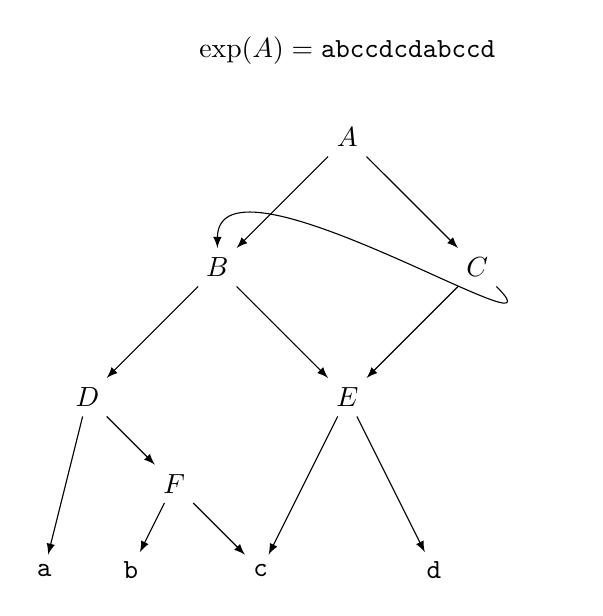
\begin{tikzpicture}[scale=0.55, y=-1cm]
                    \bigpicture{\node (txt) at (0, -2) {$\exp(A) = \mathtt{abccdcdabccd}$};

\node (A) at (0, 0) {$A$};
\node (B) at (-3, 3) {$B$};
\node (C) at (3, 3) {$C$};
\node (D) at (-6, 6) {$D$};
\node (E) at (0, 6) {$E$};
\node (F) at (-4, 8) {$F$};
\node (a) at (-7, 10) {$\mathtt{a}$};
\node (b) at (-5, 10) {$\mathtt{b}$};
\node (c) at (-2, 10) {$\mathtt{c}$};
\node (e) at (2, 10) {$\mathtt{d}$};

\draw[-latex] (A) -- (B);
\draw[-latex] (A) -- (C);
\draw[-latex] (B) -- (D);
\draw[-latex] (B) -- (E);
\draw[-latex] (C) -- (E);
\draw[-latex] (C) to [out=315,in=90] (B);
\draw[-latex] (D) -- (F);
\draw[-latex] (D) -- (a);
\draw[-latex] (F) -- (b);
\draw[-latex] (F) -- (c);
\draw[-latex] (E) -- (c);
\draw[-latex] (E) -- (e);
}
            \end{tikzpicture}
        \end{column}
    \end{columns}
  \end{frame}



  \begin{frame}<2->{Using Weight-Balanced SLPs to Initialize Boxes}
    \begin{columns}
        \begin{column}{0.5\textwidth}
            \begin{itemize}
                %\item<1> Weight-balanced SLPs do not have such rigid level structure as weight-balanced B-trees used in \where{C\textbf{K}M20}.
                \item<2-> To compute the distance matrix, use the production of the longer symbol and recurse on the two ``halves'' of the box.
                \begin{itemize}
                    \item<9-> $1 / 4 \le \len(A) / \len(B) \le 4$ for all recursive calls $(A ,B)$.
                \end{itemize}
                \item<10-> It is sufficient to maintain distance matrices for all pairs of symbols $(A, B)$ with $1 / 4 \le \len(A) / \len(B) \le 4$.
                \item<11-> Time complexity:
                \begin{itemize}
                    \item<11-> $\tOh(k)$ time per new symbol.
                    \item<11-> $\tOh(k)$ new symbols in total.
                    \item<11-> Initialization time: $\tOh(k^2)$.
                    \item<11-> Amortized over $\Theta(k)$ updates: $\tOh(k)$.
               \end{itemize}
            \end{itemize}
        \end{column}
        \begin{column}{0.5\textwidth}
            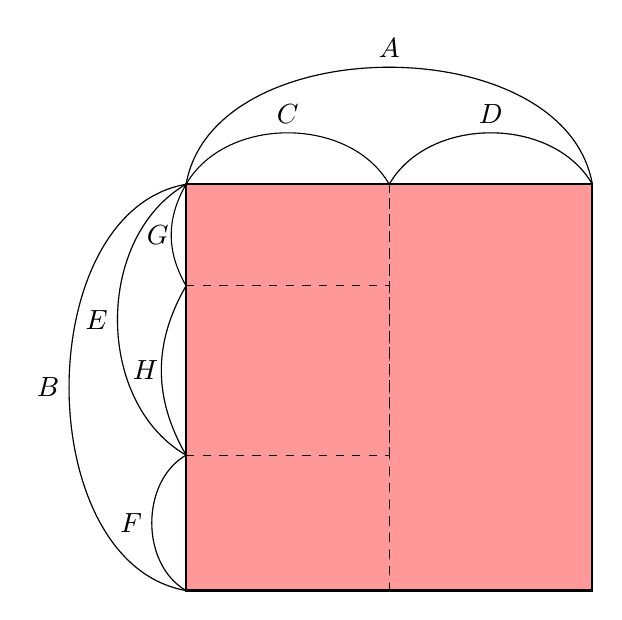
\begin{tikzpicture}[scale=0.43, y=-1cm]
                    \bigpicture{

\def\W{12}
\def\H{12}
\def\cnt{6}
\def\sizeofdot{2pt}
\def\gp{0}
%\draw[black,thin] (-1,-1) grid (\H + 1,\W + 1);

\draw<-3>[red!40, fill=red!40] (0, 0) rectangle (\H, \W);
\draw<4-5>[red!40, fill=red!40] (0, 0) rectangle (\H / 2, \W);
\draw<6-7>[red!40, fill=red!40] (0, 2*\W / 3) rectangle (\H / 2, 0);
\draw<8->[red!40, fill=red!40] (0, 0) rectangle (\H / 2, \W / 4);

\draw<-3>[thick] (0, 0) rectangle (\H, \W);
\draw<4->[thick, nearly transparent] (0, 0) rectangle (\H, \W);

\draw<-3> (0, -\gp) to [out=80,in=100] node[midway,above] {$A$} (\H, -\gp);
\draw<4->[nearly transparent] (0, -\gp) to [out=80,in=100] node[midway,above] {$A$} (\H, -\gp);

\draw<3-> (0, -\gp) to [out=60,in=120] node[midway,above] {$C$} (\H / 2, -\gp);
\draw<3> (\H / 2, -\gp) to [out=60,in=120] node[midway,above] {$D$} (\H, -\gp);
\draw<4->[nearly transparent] (\H / 2, -\gp) to [out=60,in=120] node[midway,above] {$D$} (\H, -\gp);

\draw<-5> (-\gp, 0) to [out=190,in=170] node[midway,left] {$B$} (-\gp, \W);
\draw<6->[nearly transparent] (-\gp, 0) to [out=190,in=170] node[midway,left] {$B$} (-\gp, \W);

\draw<5> (-\gp, 2*\W/3) to [out=210,in=150] node[midway,left] {$F$} (-\gp, \W);
\draw<6->[nearly transparent] (-\gp, 2*\W/3) to [out=210,in=150] node[midway,left] {$F$} (-\gp, \W);

\draw<5-7> (-\gp, 0) to [out=210,in=150] node[midway,left] {$E$} (-\gp, 2*\W / 3);
\draw<8->[nearly transparent] (-\gp, 0) to [out=210,in=150] node[midway,left] {$E$} (-\gp, 2*\W / 3);

\draw<7-> (-\gp, 0) to [out=240,in=120] (-\gp, \W / 4);
\node<7-> (G) at (-0.84, \W / 8) {$G$};

\draw<7> (-\gp, \W / 4) to [out=240,in=120] (-\gp, 2*\W/3);
\node<7> (H) at (-1.2, 11*\W / 24) {$H$};
\draw<8->[nearly transparent] (-\gp, \W / 4) to [out=240,in=120] (-\gp, 2*\W/3);
\node<8->[nearly transparent] (H) at (-1.2, 11*\W / 24) {$H$};

\draw<3-5>[dashed] (\H / 2, 0) -- (\H / 2, \W);
\draw<6->[dashed, nearly transparent] (\H / 2, \W) -- (\H / 2, 2*\W / 3);
\draw<3-5>[thick] (\H / 2, 0) -- (0, 0) -- (0, \W) -- (\H / 2, \W);
\draw<6-7>[dashed] (\H / 2, 2*\W / 3) -- (\H / 2, 0);
\draw<8->[dashed, nearly transparent] (\H / 2, \W / 4) -- (\H / 2, \W);
\draw<8->[dashed, nearly transparent] (\H / 2, \W / 4) -- (\H / 2, \W);
\draw<6-7>[thick] (0, 2*\W / 3) -- (0, 0) -- (\H / 2, 0);
\draw<8->[thick] (\H/2, 0) -- (0, 0) -- (0, \W / 4);
\draw<8->[dashed] (\H / 2, 0) -- (\H / 2, \W / 4);
\draw<5-7>[dashed] (0, 2*\W / 3) -- (\H / 2, 2*\W / 3);
\draw<8->[dashed,nearly transparent] (0, 2*\W / 3) -- (\H / 2, 2*\W / 3);
\draw<7->[dashed] (0,  \W / 4) -- (\H / 2, \W / 4);
}
            \end{tikzpicture}
            %*Picture of a part of the box for a recursive call and how we recurse further*
        \end{column}
    \end{columns}
  \end{frame}

  

  \begin{frame}{Using Weight-Balanced SLPs to Initialize Boxes}
   \begin{columns}
       \begin{column}{0.5\textwidth}
           \begin{itemize}
               \item<1-> For a fixed $A$, there are $\Oh(k / \len(A))$ symbols $B$ with $1 / 4 \le \len(A) / \len(B) \le 4$.
               \item<7-> If $B\to B_LB_R$, then computing the distance matrix for $(A,B)$ from the distance matrices of $(A,B_L)$ and $(A,B_R)$ takes $\tOh(\len(A))$ time.
               \item<8-> Each update (copy-paste, edit, substring extraction) takes $\tOh(k)$ time:
               \begin{itemize}
                   \item $\tOh(1)$ new symbols per update.
                   \item $\tOh(k / \len(A) \cdot \len(A)) = \tOh(k)$ time per new symbol $A$.
               \end{itemize} 
               \item<9-> Initializing boxes takes $\tOh(k)$ updates.
               \begin{itemize}
                   \item<10-> Initialization time: $\tOh(k^2)$.
                   \item<10-> Amortized update time: $\tOh(k)$.
              \end{itemize}

           \end{itemize}
       \end{column}
       \begin{column}{0.5\textwidth}
           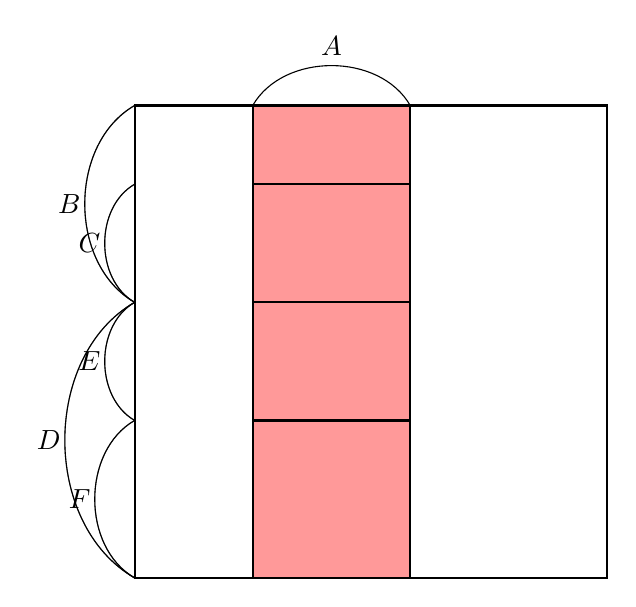
\begin{tikzpicture}[scale=0.5, y=-1cm]
                   

\def\W{12}
\def\H{12}
\def\cnt{6}
\def\sizeofdot{2pt}
\def\gp{0.0}
\def\lx{3}
\def\rx{7}
%\draw[black,thin] (-1,-1) grid (\H + 1,\W + 1);



\foreach \iter/\ly/\ry/\cursym in {2/0/5/B,3/2/5/C,4/5/12/D,5/5/8/E,6/8/12/F}
    \draw[white] (-\gp, \ly) to [out=210,in=150] node[midway,left=-2] {$\cursym$} (-\gp, \ry);

\foreach \iter/\ly/\ry/\cursym in {2/0/5/B,3/2/5/C,4/5/12/D,5/5/8/E,6/8/12/F}{
    \draw<\iter> (-\gp, \ly) to [out=210,in=150] node[midway,left=-2] {$\cursym$} (-\gp, \ry);
    \draw<\iter->[semitransparent] (-\gp, \ly) to [out=210,in=150] (-\gp, \ry);
    \draw<\iter>[thick,fill=red!40] (\lx, \ly) rectangle (\rx, \ry);
    \draw<\iter->[dashed,semitransparent] (\lx, \ly) rectangle (\rx, \ry);
};

\draw[thick] (0, 0) rectangle (\H, \W);
\draw (\lx, -\gp) to [out=60,in=120] node[midway,above] {$A$} (\rx, -\gp);

           \end{tikzpicture}
           %*Picture of SLPs of two fragments of a box, and to which things one symbol is mapped*
       \end{column}
   \end{columns}
 \end{frame}

%\ end{comment}

  %\ begin{comment}

  % \begin{frame}{From Small Self-Edit Distance to the General Case}
  %   \begin{columns}
  %       \begin{column}{0.5\textwidth}
  %           \begin{itemize}
  %               \item<1-> \where{C\textbf{K}W23,GJKT24} use divide and conquer:
  %               \begin{enumerate}
  %                   \item Find out where the optimal alignment crosses the midpoint of $X$.
  %                   \item<9-> Recursively compute the two halves of the optimal alignment.
  %               \end{enumerate}
  %               \item<11-> If we make an update in $X_L$, it may affect the decomposition $Y = Y_L Y_R$, and thus affect the $(X_R, Y_R)$ recursive call.
  %           \end{itemize}
  %       \end{column}
  %       \begin{column}{0.5\textwidth}
  %           \hfill
  %           \begin{tikzpicture}[scale=0.5, y=-1cm]
  %                   \bigpicture{
  %                       

\def\W{12}
\def\H{12}
\def\cnt{6}
\def\sizeofdot{4pt}
\def\gp{0.0}
%\draw[black,thin] (-1,-1) grid (\H + 1,\W + 1);



\draw[line width=3pt, white, line cap=round] (0, 0) -- (1, 1) -- (1, 2) -- (4, 5) -- (5.5, 5) -- (6.5, 6) -- (6.5, 8) -- (9, 10.5) -- (10.5, 10.5) -- (\H, \W);

%\draw<-4>[dashed, gray] (0, 0) -- (\H, \W);


\node<1>[white] (XL) at (\H / 5, -1) {\Large $X_L$};
\node<2-> (XL) at (\H / 5, -1) {\Large $X_L$};
\node<2-> (XR) at (4 * \H / 5, -1) {\Large $X_R$};

\draw<4-8>[latex-latex] (\H / 3, -0.3) to node[midway, above] {$\sed = \Theta(k)$} (2 * \H / 3, -0.3);
\draw<4-8>[latex-latex] (\H / 3, -0.3) -- (\H / 2, -0.3); 
\draw<4-8>[latex-latex] (2*\H / 3, -0.3) -- (\H / 2, -0.3); 
\draw<4-8>[dashed, gray] (\H / 3, 0) -- (\H / 3, \W);
\draw<4-8>[dashed, gray] (2 * \H / 3, 0) -- (2 * \H / 3, \W);


%\draw<11->[line width=2pt, blue!30,line cap=round] (\H / 3, \W / 3) -- (4, 5.5) -- (5.5, 7) -- (6.5, 7) -- (7.5,8) -- (2 * \H / 3, 2 * \W / 3);

%\draw<6>[line width=3pt, darkgreen!70, semitransparent, line cap=round] (0, 0) -- (1, 1) -- (1, 2) -- (3.5, 4.5) -- (5.5, 4.5) -- (7, 6) -- (7, 8.5) -- (9, 10.5) -- (10.5, 10.5) -- (\H, \W);

\draw<3-6>[line width=3pt, darkgreen!70, semitransparent, line cap=round] (0, 0) -- (1, 1) -- (1, 2) -- (3.5, 4.5) -- (5, 4.5) -- (6.5, 6) -- (6.5, 7) -- (7,7.5) -- (7, 8.5) -- (9, 10.5) -- (10.5, 10.5) -- (\H, \W);

\draw<6-8>[line width=2pt, blue!30,line cap=round] (\H / 3, \W / 3) -- (4.5, 4) -- (6.5, 6) -- (6.5, 7) -- (7.5,8) -- (2 * \H / 3, 2 * \W / 3);

%\node<6-7>[circle,draw=blue, fill=blue, inner sep=0pt,minimum size=2pt] (dd) at (5, 4.5) {};
%\node<6-7>[circle,draw=blue, fill=blue, inner sep=0pt,minimum size=2pt] (ddd) at (7, 7.5) {};

%\draw<6-8>[line width=2pt, blue!30,line cap=round,nearly transparent] (0, 0) -- (1, 1) -- (1, 2) -- (3,4) -- (4,4) (8,8) -- (8,9.5) -- (9, 10.5) -- (10.5, 10.5) -- (\H, \W);

\draw<8-12>[dashed, gray] (0, 5.5) -- (\H, 5.5);

\draw<10>[very thick, violet, fill=violet, fill opacity=0.2] (0, 0) rectangle (\H / 2, 5.5);
\draw<11>[very thick, violet, fill=violet, fill opacity=0.2] (\H / 2, 5.5) rectangle (\H, \W);

\draw<10>[line width=2pt, darkgreen!70, line cap=round] (0, 0) -- (1, 1) -- (1, 2) -- (3.5, 4.5) -- (5, 4.5) -- (6, 5.5);
\draw<11-12>[line width=2pt, darkgreen!70, line cap=round](0, 0) -- (1, 1) -- (1, 2) -- (3.5, 4.5) -- (5, 4.5) -- (6.5, 6) -- (6.5, 7) -- (7,7.5) -- (7, 8.5) -- (9, 10.5) -- (10.5, 10.5) -- (\H, \W);


\draw<13->[line width=3pt, darkgreen!70, semitransparent, line cap=round] (0, 0) -- (0.5, 0) -- (2.5, 2) -- (3.5, 2) -- (5.5, 4) -- (5.5, 6.5) -- (6, 7) -- (7, 7) -- (7.5, 7.5) -- (9, 7.5) -- (11, 9.5) -- (11, 11) -- (\H, \W);

\draw<13->[dashed, gray] (0, 7) -- (\H, 7);
\draw<14>[very thick, violet, fill=violet, fill opacity=0.2] (0, 0) rectangle (\H / 2, 7);
\draw<15>[very thick, violet, fill=violet, fill opacity=0.2] (\H / 2, 7) rectangle (\H, \W);

\node<3->[circle,draw=darkgreen, fill=darkgreen, inner sep=0pt,minimum size=\sizeofdot] (olddot) at (\H / 2, 5.5) {};
%\node<13->[circle,draw=darkgreen, fill=darkgreen, inner sep=0pt,minimum size=\sizeofdot] (olddot) at (\H / 2, 7) {};

\draw[thick] (0, 0) rectangle (\H, \W);
\draw<5-8>[blue, thick] (\H / 3, \W / 3) rectangle (2 * \H / 3, 2 * \W / 3);
\draw<2-> (\H / 2, 0) -- (\H / 2, \W);

%\draw<11->[fill=orange,thin,opacity=0.4] (5 * \H / 12, 0) rectangle (5 * \H / 12 + 0.125, \W);

  %                   }
  %           \end{tikzpicture}
  %           \hfill
  %           %*Picture how small $\sed$ region in the middle gives the middle point and how the opt alignment intersects the small $\sed$ alignment; and how a change in $X_L$ may affect $Y_R$*
  %       \end{column}
  %   \end{columns}
  % \end{frame}

 % \ end{comment}

 \begin{frame}{Self-Edit Distance vs Alignment Intersections}
  \begin{columns}
      \begin{column}{0.5\textwidth}
          \begin{block}{Observation\hfill [C\textbf{K}W23]}
              Two alignments $X \onto Y$ of cost at most $k$ \textbf{must intersect} within \emph{every} fragment of $X$ of self-edit distance $> 2k$.
          \end{block}
      \end{column}
      \begin{column}{0.5\textwidth}
          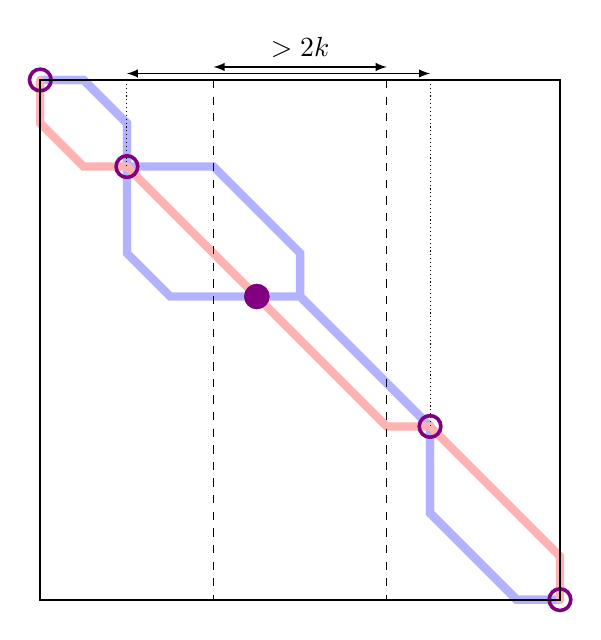
\begin{tikzpicture}[scale=0.55, y=-1cm]
              \bigpicture{
\def\shft{0}
\def\W{12}
\def\H{12}
\def\myi{2}
\def\cnt{6}
\def\gp{2}
%\draw[black,thin] (-1,-1) grid (\H + 1,\W + 1);




\draw<4-5>[line width=3pt, blue!30!,line cap=round] (0, 0) -- (1, 0) -- (2, 1) -- (2,2) -- (4, 2) -- (5, 3) -- (6,4)-- (6, 5) -- (9, 8) -- (9, 10) -- (11, 12) -- (12, 12);
\draw<6->[line width=3pt, blue!30!,line cap=round] (0, 0) -- (1, 0) -- (2, 1) -- (2,2) -- (2, 4) -- (3, 5) -- (6, 5) -- (9, 8) -- (9, 10) -- (11, 12) -- (12, 12);
\draw[line width=3pt, red!30,line cap=round] (0, 0) -- (0, 1) -- (1, 2) -- (2, 2) -- (8, 8) -- (9, 8) -- (12, 11) -- (12, 12);

\draw[dashed] (\H / 3, 0) -- (\H / 3, \W);
\draw[dashed] (2 * \H / 3, 0) -- (2 * \H / 3, \W);

\draw<5-6>[densely dotted] (2, 0) -- (2,2);
\draw<5-6>[densely dotted] (9, 0) -- (9,8);


\draw[latex-latex] (\H / 3, -0.3) --node[above]{$\sed > 2k$} (2 * \H / 3, -0.3);
\draw<5-6>[latex-latex] (2, -0.15) -- (9, -0.15);

\draw [line width=1.3pt, violet] (0,0) circle [radius=.25];
\draw [line width=1.3pt, violet] (2, 2) circle [radius=.25];
\draw<6> [line width=1.3pt, violet] (5, 5) circle [radius=.25];
\draw<7> [line width=1.3pt, violet, fill=violet] (5, 5) circle [radius=.25];
\draw [line width=1.3pt, violet] (9, 8) circle [radius=.25];
\draw [line width=1.3pt, violet] (\H,\W) circle [radius=.25];


\draw[thick] (0, 0) rectangle (\H, \W);
}
          \end{tikzpicture}
      \end{column}
  \end{columns}
\end{frame}

  \begin{frame}[label=current]{Summary}
  \begin{alertblock}{Theorem}
    There is a dynamic algorithm that maintains $\ed(X,Y)$ subject to edits in $X$ and $Y$, taking $\Oh(k\log^4 n)$ time per update, where $n=|X|+|Y|$ and $k=\ed(X,Y)$.
  \end{alertblock}

  \medskip
  \pause
  \textbf{Open problem:}
  \begin{itemize}
    \item Reduce the $\log^4 n$ factor to $\log^2 n$ and beyond.
  \end{itemize}

  \pause
  \medskip
  \textbf{Weighted edit distance:}
    \begin{itemize}
      \item<3-> Static algorithms:
      \begin{itemize}
        \item<3-> $\Ohtilde(n+\sqrt{nk^3})$ for arbitrary normalized weights (tight if $\sqrt{n}\le k \le n$);\hfill \where{C\textbf{K}W23}
        \item<4-> $\Ohtilde(n+k^{2.5})$ for integer weights;\hfill \where{this work}
        \item<5-> $\Ohtilde(n+Wk^2)$ for weights in $[0\dd W]$.\hfill \where{this work}
      \end{itemize}
      \item<6-> Dynamic algorithms:
      \begin{itemize}
        \item<6-> $\Ohtilde(k^3)$ for arbitrary normalized weights;
        \item<6-> $\Ohtilde(k^{2.5})$ for integer weights;
        \item<6-> \alt<-6>{$\Ohtilde(Wk^2)$}{{\boldmath$\Ohtilde(W^2k)$}} for weights in $[0\dd W]$.\only<7->{\hfill \where{this work}}
      \end{itemize}
    \end{itemize}

    \begin{tikzpicture}[overlay,remember picture]
      \node<8->[text=MPIgreen] at ([xshift=3.75cm,yshift=.8cm]current page.center){\Huge Thank you!};
      \end{tikzpicture}%
\end{frame}
\end{comment}
